\documentclass[prx,twocolumn,superscriptaddress,longbibliography,floatfix]{revtex4-2}

\usepackage{amsmath,amssymb,amsfonts}
\usepackage{graphicx}
\usepackage{hyperref}
\usepackage{braket}
\usepackage{booktabs}
\usepackage{multirow}
\usepackage{makecell}
\usepackage{xcolor}
\usepackage{float}
\usepackage{tikz}
\usetikzlibrary{quantikz2,decorations.pathreplacing,calc}

\newcommand{\CC}{\mathcal{C}}
\newcommand{\DD}{\mathcal{D}}
\newcommand{\EE}{\mathcal{E}}
\newcommand{\UU}{\mathcal{U}}
\newcommand{\tr}{\mathrm{Tr}}
\newcommand{\Frec}{F_\mathrm{rec}}
\newcommand{\Fest}{F_\mathrm{est}}
\newcommand{\Fnoisy}{F_\mathrm{noisy}}
\newcommand{\rhot}{\rho_\mathrm{target}}
\newcommand{\rhon}{\rho_\mathrm{noisy}}
\newcommand{\rhor}{\rho_\mathrm{rec}}
\newcommand{\rhoe}{\hat{\rho}_\mathrm{est}}

\begin{document}

\title{Blind Catalytic Quantum Error Correction:\\
Target-State Estimation and Fidelity Recovery Without \textit{A Priori} Knowledge}

\author{Hikaru Wakaura}
\email{h.wakaura@qiri.co.jp}
\affiliation{QIRI (Quantum Integrated Research Institute Inc.), Tokyo 107-0061, Japan}

\author{Taiki Tanimae}
\email{t.tanimae@qiri.co.jp}
\affiliation{QIRI (Quantum Integrated Research Institute Inc.), Tokyo 107-0061, Japan}

\date{\today}

\begin{abstract}
Catalytic quantum error correction (CQEC) recovers quantum states via catalytic covariant transformations but requires full knowledge of the target state.
We introduce \emph{blind CQEC}, which estimates the target from the noisy output alone before catalytic recovery.
Five estimation strategies are benchmarked across three noise models (dephasing, depolarizing, amplitude damping), four quantum algorithms ($d = 4$--$64$), Haar-random states up to $d = 256$, and mixed-state targets with variable purity.
Key results: (i)~coherence maximization achieves $\Frec > 0.95$ for $d \leq 16$ without noise-model knowledge, matching the oracle to within $4\%$; (ii)~channel inversion is required at $d = 64$ ($\Frec = 0.905$); (iii)~estimation and recovery fidelities are linearly correlated ($r > 0.99$), identifying target estimation as the sole bottleneck; (iv)~an analytical crossover dimension $d^* \approx 25$--$40$ separates noise-model-free and noise-informed regimes, bridged by a hybrid interpolation strategy; (v)~copy scaling follows $1 - F(n) \sim n^{-\alpha}$ with $\alpha \in [0.4, 2.2]$, spanning the statistical averaging and denoising synergy limits.
Direct comparison with standard quantum error mitigation (ZNE, PEC, virtual distillation) shows that blind coherence maximization uniquely achieves state-level recovery without noise-model knowledge, while blind channel inversion matches PEC's fidelity at single-copy overhead.
An end-to-end VQE demonstration for H$_2$ shows $3.4\times$ energy-error reduction with channel-inversion blind CQEC, and a circuit-level sanity check on \texttt{qiskit-aer} confirms that the density-matrix predictions translate to small noisy circuits.
We also derive an analytical Lipschitz bound $\Frec \geq 1 - 2\|\rhoe - \rhot\|_1$ for the density-matrix-level recovery map, providing the theoretical underpinning for the empirical estimation--recovery correlation.
\end{abstract}

\maketitle


%% ============================================================
\section{Introduction}
\label{sec:introduction}

Catalytic quantum error correction (CQEC), introduced in Ref.~\cite{Wakaura2026unified}, exploits the arbitrary amplification of quantum coherence under catalytic covariant transformations~\cite{Shiraishi2024} to recover quantum states corrupted by decoherence.
Unlike conventional quantum error correction (QEC), which requires encoding overhead and fails above a noise threshold~\cite{Shor1995,Gottesman1997,Knill2005}, CQEC is threshold-free: recovery succeeds whenever the coherent modes of the target state are present in the noisy state, $\CC(\rhot) \subseteq \CC(\rhon)$, regardless of how small the residual coherence is~\cite{Shiraishi2024}.
The catalyst is reusable across unlimited correction cycles~\cite{Wakaura2026unified,Wakaura2026catalyst}.

However, CQEC in its original formulation requires \emph{complete knowledge of the target state} $\rhot$.
This requirement is restrictive: in many practically relevant scenarios---most notably variational quantum algorithms where noisy intermediate circuit outputs must be improved without knowledge of the ideal state~\cite{Peruzzo2014,Cerezo2021}, and iterative quantum algorithms where the target evolves across rounds---the ideal output state is unknown to the error correction module.
The target-state requirement has been identified as the principal conceptual gap between CQEC and conventional QEC~\cite{Wakaura2026unified}.

In this work, we substantially relax this requirement by introducing \emph{blind CQEC},\footnote{We use ``blind'' in the operational sense that the target state is unknown to the correction protocol, distinct from blind quantum computing, which concerns hiding computation from an untrusted server.} where the target state $\rhot$ is estimated from the noisy state $\rhon$ (or multiple noisy copies) before catalytic correction.
We frame the problem as a two-stage protocol:
\begin{enumerate}
\item \emph{Estimation:} Construct an estimate $\rhoe$ from $\rhon$ and any available side information (noise model, copy count).
\item \emph{Correction:} Apply standard CQEC with $\rhoe$ as the proxy target.
\end{enumerate}
The central question is: \emph{how close can $\Frec = F(\rhor, \rhot)$ approach the oracle fidelity when the target is unknown?}

The nontrivial content of this question is twofold.
First, it is not \emph{a priori} clear that CQEC is robust to estimation error: the catalytic amplification protocol involves a nonlinear sequence of coherence transfers whose sensitivity to the target specification has not been analyzed.
Second, while one could in principle apply any quantum state estimation method~\cite{Hradil1997,Gross2010,Haah2017} before CQEC, the interplay between the estimation strategy and the subsequent catalytic recovery creates structure-specific constraints (e.g., the mode inclusion condition must hold for $\rhoe$, not just $\rhot$) that generic estimators do not address.

We developed five estimation strategies with varying information requirements (Table~\ref{tab:strategies}) and benchmarked them across four quantum algorithms from recent literature~\cite{Chen2021,Ivashkov2024,Clinton2026,Regev2024}, three noise channels, and Hilbert space dimensions $d = 4$--$64$, characterizing the copy scaling of blind CQEC in the resource-constrained regime.

Our main results established three regimes:
\begin{itemize}
\item \emph{Low-dimensional ($d \leq 16$), unknown noise model.} Coherence maximization---a strategy requiring no explicit noise-model specification, though implicitly favoring phase-preserving channels---achieves $\Frec > 0.95$, within $0.5$--$4\%$ of the oracle.
\item \emph{High-dimensional ($d = 64$), known noise model.} Noise-channel inversion is required, achieving $\Frec \approx 0.91$ under combined noise.
\item \emph{Copy-constrained regime.} As few as $n = 5$--$10$ copies suffice for $\Frec > 0.95$ at $d \leq 16$; scaling exponents $\alpha$ range from $0.4$ (dephasing) to $2.2$ (amplitude damping inversion).
\end{itemize}


%% ============================================================
\section{Theoretical Background}
\label{sec:theory}

\subsection{Catalytic covariant transformations}
\label{sec:catalytic}

We briefly recall the framework of Refs.~\cite{Shiraishi2024,Wakaura2026unified}.
A covariant operation satisfies $\Lambda \circ \UU_t = \UU_t \circ \Lambda$ for all $t$, where $\UU_t(\rho) = e^{-iHt}\rho\,e^{iHt}$.
The modes of asymmetry $\DD(\rho) = \{\Delta_{ij} = E_i - E_j \mid \rho_{ij} \neq 0\}$ characterize the coherence structure.
The resonant coherent modes $\CC(\rho) = \langle \DD(\rho) \rangle_\mathbb{Z}$ form the integer lattice generated by $\DD(\rho)$.

\noindent\textbf{Theorem 1} (Shiraishi--Takagi~\cite{Shiraishi2024}).---\textit{%
A catalytic covariant transformation $\rho \otimes c \mapsto \tau$ with $\tr_C[\tau] = \rho'$, $\tr_S[\tau] = c$ exists if and only if $\CC(\rho') \subseteq \CC(\rho)$ and $\rho$ is full rank.}

The CQEC protocol~\cite{Wakaura2026unified} applies Theorem~1 as follows: given a noisy state $\rhon = \EE(\rhot)$ and a catalyst $c$, find a covariant map $\Lambda$ such that $\Lambda(\rhon \otimes c) = \tau$ with $\tr_C[\tau] \approx \rhot$.
This requires knowing $\rhot$ explicitly to construct $\Lambda$.
Note that Theorem~1 requires the input state to be full rank.
In our benchmarks, this condition is satisfied: depolarizing noise ($\rho \mapsto (1-p)\rho + pI/d$) always produces full-rank states, and the combined noise model includes a depolarizing component.
For pure dephasing alone, the diagonal elements are unchanged and rank is preserved from the target; in practice, any finite-temperature environment ensures full rank through thermal population of all levels.

\subsection{Implementation via density-matrix simulation}
\label{sec:implementation}

In our numerical benchmarks, the CQEC recovery is implemented via the ICEC protocol of Ref.~\cite{Wakaura2026unified}, which operates at the density-matrix level.
Given $\rhon$ and a target estimate $\rhoe$, the protocol:
(i)~verifies the mode inclusion condition $\CC(\rhoe) \subseteq \CC(\rhon)$;
(ii)~constructs a catalyst state $c$ with coherent modes $\CC(c) \supseteq \CC(\rhoe)$;
(iii)~applies the catalytic covariant transformation on $\rhon \otimes c$ to produce a state whose partial trace over the catalyst subspace approximates $\rhoe$.
All operations are performed as $d \times d$ matrix manipulations (or $(d \cdot d_c) \times (d \cdot d_c)$ for the joint system) without circuit-level decomposition.
In our benchmarks, the catalyst dimension is $d_c = d$ (matching the system dimension), following the construction of Ref.~\cite{Wakaura2026unified}.
The dominant computational cost of the recovery step is therefore $O(d^3)$ for eigendecomposition and $O(d^6)$ for the joint-system operations (since the joint Hilbert space has dimension $d \cdot d_c = d^2$).
At $d = 64$, this corresponds to $4096 \times 4096$ matrices, which remain tractable for density-matrix simulation but would become prohibitive for $d \gg 10^3$ without exploiting tensor product structure.
This approach is exact for the density-matrix-level physics but does not address gate compilation overhead or decoherence during the recovery itself, which we leave to future work (Sec.~\ref{sec:limitations}).

\subsection{The target-knowledge bottleneck}
\label{sec:bottleneck}

In standard CQEC, the target state enters in two places:
(a)~the mode inclusion check $\CC(\rhot) \subseteq \CC(\rhon)$;
(b)~the construction of the catalytic map $\Lambda$, which steers amplification toward the off-diagonal structure of $\rhot$.
Without $\rhot$, neither step can be performed exactly.

In blind CQEC, we replace $\rhot$ by an estimate $\rhoe$ and accept a fidelity penalty.
To quantify this, we use the bound $1 - F(\rho,\sigma) \leq \|\rho - \sigma\|_1$ (which follows from the Fuchs--van de Graaf inequality~\cite{FuchsGraaf1999} for the squared-fidelity convention of Eq.~\eqref{eq:fidelity}) and the triangle inequality for the trace norm.
Let $\Frec^{(\mathrm{oracle})}$ denote the recovery fidelity when the true target $\rhot$ is known.
For a fixed catalyst state and dimension, the ICEC protocol defines a family of CPTP maps $\{\Lambda_\sigma\}$ parameterized by the target specification~$\sigma$.
The recovery map $\Lambda_\sigma$ is a valid quantum channel for each~$\sigma$, and the Lipschitz continuity of the protocol in the target parameter---which we verify numerically (Sec.~\ref{sec:correlation})---implies
$\|\Lambda_{\rhoe}(\rhon) - \Lambda_{\rhot}(\rhon)\|_1 \leq L\,\|\rhoe - \rhot\|_1$
for a protocol-dependent Lipschitz constant $L \leq 1$ (observed empirically; see Eq.~\eqref{eq:correlation}).
Combining:
\begin{equation}
\Frec \geq \Frec^{(\mathrm{oracle})} - L\,\|\rhoe - \rhot\|_1,
\label{eq:fidelity_penalty}
\end{equation}
where $L \leq 1$ is the Lipschitz constant of the recovery map with respect to the target specification.
For single-copy strategies (coherence maximization, channel inversion), $\rhoe$ is deterministic and Eq.~\eqref{eq:fidelity_penalty} applies directly with $\|\rhoe - \rhot\|_1$ being the systematic estimation error.
For multi-copy averaging with $n$ copies, $\rhoe$ is itself a random variable whose trace-distance error decomposes as $\|\rhoe - \rhot\|_1 \leq \|\overline{\rhoe} - \rhot\|_1 + O(n^{-1/2})$, where $\overline{\rhoe} = \mathbb{E}[\rhoe]$ is the systematic bias and the $O(n^{-1/2})$ term captures finite-copy statistical fluctuations.
Substituting into Eq.~\eqref{eq:fidelity_penalty}:
\begin{equation}
\Frec \geq \Frec^{(\mathrm{oracle})} - L\bigl(\|\overline{\rhoe} - \rhot\|_1 + O(n^{-1/2})\bigr).
\label{eq:fidelity_penalty_multicopy}
\end{equation}
The two error sources are: \emph{estimation bias} $\|\overline{\rhoe} - \rhot\|_1$ (systematic, strategy-dependent) and \emph{finite-copy variance} (statistical, relevant only for multi-copy strategies, vanishing as $n \to \infty$).
We emphasize that the bound~\eqref{eq:fidelity_penalty} is semi-empirical: the Lipschitz continuity is verified numerically ($L \approx 0.98$, Sec.~\ref{sec:correlation}) rather than proven analytically for the ICEC protocol in general.
Eq.~\eqref{eq:fidelity_penalty} motivates our approach: minimizing the estimation error $\|\rhoe - \rhot\|_1$ directly maximizes recovery fidelity.

\subsection{Analytical Lipschitz continuity of the recovery map}
\label{sec:lipschitz_proof}

The empirical Lipschitz constant $L \approx 0.98$ observed in Sec.~\ref{sec:correlation} can in fact be obtained analytically for the density-matrix-level ICEC implementation used throughout this work.
At the density-matrix level, the recovery map produces $\rhor = \Pi(\rhoe)$, where
\begin{equation}
\Pi(X) = \frac{X_+}{\tr X_+},\qquad X_+ \equiv \sum_i \max(0,\lambda_i)\,|v_i\rangle\!\langle v_i|,
\label{eq:psd_proj}
\end{equation}
is the spectral projection onto the PSD cone followed by trace renormalization, with $\{(\lambda_i, v_i)\}$ the spectral decomposition of the Hermitian part of~$X$.
For the oracle target $\rhot$, which is already PSD with unit trace, $\Pi(\rhot) = \rhot$.

\noindent\textbf{Lemma 1} (Lipschitz continuity of $\Pi$ in trace norm).---\textit{%
For Hermitian matrices $A, B$ with $\tr A = \tr B = 1$,
\begin{equation}
\|\Pi(A) - \Pi(B)\|_1 \leq 2\,\|A - B\|_1.
\label{eq:lemma_lipschitz}
\end{equation}
}

\noindent\textit{Proof.}
Eigenvalue clipping $\lambda_i \mapsto \max(0, \lambda_i)$ is 1-Lipschitz on $\mathbb{R}$ and the spectral function $A \mapsto A_+$ inherits this property in any unitarily invariant norm by Lidskii's inequality~\cite{NielsenChuang2010}: $\|A_+ - B_+\|_1 \leq \|A - B\|_1$.
Let $t_A = \tr A_+$ and $t_B = \tr B_+$.
Since $\tr A = \tr B = 1$ and the negative parts $A_- = A_+ - A$, $B_- = B_+ - B$ satisfy $\|A_-\|_1 = t_A - 1$ (and similarly for~$B$), we have $|t_A - t_B| \leq \|A - B\|_1$ by the triangle inequality.
Decomposing
\begin{align}
\Pi(A) - \Pi(B) &= \tfrac{1}{t_A}A_+ - \tfrac{1}{t_B}B_+ \nonumber\\
&= \tfrac{1}{t_A}(A_+ - B_+) + \bigl(\tfrac{1}{t_A} - \tfrac{1}{t_B}\bigr)B_+,
\end{align}
and using $\|B_+\|_1 = t_B$, $t_A, t_B \geq 1$ (since $\tr A_+ \geq \tr A = 1$):
\begin{equation}
\|\Pi(A) - \Pi(B)\|_1 \leq \tfrac{1}{t_A}\|A - B\|_1 + \tfrac{|t_A - t_B|}{t_A} \leq 2\|A - B\|_1.
\end{equation}
\hfill$\square$

\noindent\textbf{Corollary} (Recovery-fidelity bound).---\textit{For the density-matrix-level ICEC, the bound~\eqref{eq:fidelity_penalty} holds with explicit Lipschitz constant $L \leq 2$:
\begin{equation}
\Frec \geq 1 - 2\|\rhoe - \rhot\|_1.
\label{eq:explicit_bound}
\end{equation}
}
This follows from Lemma~1 combined with $1 - F(\rhor, \rhot) \leq \|\rhor - \rhot\|_1 = \|\Pi(\rhoe) - \Pi(\rhot)\|_1$ (Fuchs--van de Graaf~\cite{FuchsGraaf1999} for the squared-fidelity convention).

The bound $L \leq 2$ is loose: the empirical $L \approx 0.98$ corresponds to the regime where $\rhoe$ is itself nearly PSD with $t_A \approx 1$, in which case both terms in the proof reduce to $\|A - B\|_1$ scaled by $t_A^{-1} \approx 1$.
For circuit-level ICEC implementations~\cite{Wakaura2026unified}, the catalytic amplification step introduces additional channel non-idealities that may further weaken~$L$; we leave the analytical extension to that setting for future work.


\subsection{Analytical crossover dimension}
\label{sec:crossover_theory}

We derive an approximate crossover dimension $d^*$ at which coherence maximization and channel inversion achieve equal estimation error.
For a Haar-random pure state $|\psi\rangle$ in dimension~$d$, the expected populations scale as $\mathbb{E}[p_i] = 1/d$ with variance $\mathrm{Var}[p_i] = (d-1)/[d^2(d+1)]$~\cite{NielsenChuang2010}.
Under depolarizing noise $\EE_p$, the populations become $p_i' = (1-p)p_i + p/d$, so the estimation error for coherence maximization, which uses the physicality bound $\sqrt{p_i' p_j'}$, is dominated by the bias $|\sqrt{p_i' p_j'} - |\rho_{ij}^{\mathrm{target}}||$.

For a Haar-random pure state, $\mathbb{E}[|\rho_{ij}|^2] = 1/[d(d+1)]$ for $i \neq j$, while $\sqrt{p_i' p_j'} \approx [(1-p)/d + p/d] = 1/d$ for large~$d$.
The coherence-maximization error thus scales as $\epsilon_{\mathrm{CM}} \sim d \cdot |1/d - 1/\sqrt{d(d+1)}| \sim 1/(2d)$ per matrix element, giving a trace-norm error $\|\rhoe^{\mathrm{CM}} - \rhot\|_1 \sim O(1)$ independent of~$d$ (since there are $d^2$ elements, each contributing $\sim 1/d^2$ to the trace norm after concentration).

For channel inversion under depolarizing noise, $\rhoe^{\mathrm{inv}} = (\rhon - pI/d)/(1-p)$ is exact when $\EE$ is purely depolarizing, so $\|\rhoe^{\mathrm{inv}} - \rhot\|_1 = 0$.
Under combined noise, the residual error arises from the uncompensated components (e.g., dephasing not inverted when only depolarizing inversion is applied).
Writing the combined channel as $\EE = \EE_{\mathrm{AD}} \circ \EE_p \circ \EE_\gamma$ and inverting only approximately, the residual scales as $\epsilon_{\mathrm{inv}} \sim \gamma_{\mathrm{AD}} + \gamma/d$ (the amplitude-damping component is $d$-independent, while dephasing inversion error grows with the mode gap).

The crossover occurs when $\epsilon_{\mathrm{CM}} \approx \epsilon_{\mathrm{inv}}$, giving
\begin{equation}
d^* \approx \frac{1}{2(\gamma_{\mathrm{AD}} + \gamma/d^*)},
\label{eq:crossover}
\end{equation}
which for our combined-noise parameters ($\gamma = 1.0$, $\gamma_{\mathrm{AD}} = 0.1$) yields $d^* \approx 25$--$40$.
This is consistent with the numerically observed crossover at $d \approx 32$ (Sec.~\ref{sec:haar_sweep}).


%% ============================================================
\section{Estimation Strategies}
\label{sec:strategies}

This section presents the five estimation strategies, ordered by increasing information requirements.

\begin{table}[b]
\caption{Target-state estimation strategies for blind CQEC.
The estimation complexity column refers to the cost of constructing $\rhoe$ from $\rhon$; all strategies additionally incur $O(d^3)$ cost for the CQEC recovery step (matrix diagonalization and catalytic map construction).}
\label{tab:strategies}
\begin{ruledtabular}
\begin{tabular}{lcc}
Strategy & Info required & Est.\ complexity \\
\hline
Naive & None & $O(1)$ \\
Coherence max & None & $O(d^2)$ \\
Iterative & None & $O(k \cdot d^3)$ \\
Multi-copy avg. & $n$ copies & $O(n d^2)$ \\
Channel inversion & Noise model & $O(d^2)$ \\
\end{tabular}
\end{ruledtabular}
\end{table}


\subsection{Naive passthrough}
\label{sec:naive}

The simplest approach uses $\rhoe = \rhon$ directly.
Since $\rhon$ is the corrupted version of $\rhot$, this is equivalent to running CQEC with the ``wrong'' target.
As we show in Sec.~\ref{sec:results}, this yields $\Frec = \Fnoisy$ (no improvement), because catalytic amplification faithfully steers the state toward $\rhoe = \rhon$, which is itself the noisy state.

\subsection{Coherence maximization}
\label{sec:cohmax}

We propose maximizing the off-diagonal coherence of $\rhon$ while preserving its diagonal (population) structure:
\begin{equation}
(\rhoe)_{ij} = \begin{cases}
(\rhon)_{ii} & \text{if } i = j, \\
\sqrt{(\rhon)_{ii}\,(\rhon)_{jj}}\,e^{i\phi_{ij}} & \text{if } i \neq j,
\end{cases}
\label{eq:cohmax}
\end{equation}
where $\phi_{ij} = \arg[(\rhon)_{ij}]$ when $(\rhon)_{ij} \neq 0$, and $\phi_{ij} = 0$ otherwise (coherences that have been completely suppressed cannot be recovered by this strategy; see below).
This corresponds to constructing the \emph{most coherent state consistent with the observed populations and phases}.

The rationale is physical: decoherence reduces $|\rho_{ij}|$ below the physicality bound $\sqrt{p_i p_j}$ but preserves the phase (for dephasing and depolarizing channels).
By restoring $|\rho_{ij}|$ to its maximum allowed value, we undo the amplitude damping of coherences without requiring knowledge of the original amplitudes.

The matrix $\rhoe$ constructed by Eq.~\eqref{eq:cohmax} is Hermitian and trace-one by construction.
It is positive semidefinite when the phases $\{\phi_{ij}\}$ are consistent with a rank-one state (i.e., $\phi_{ij} = \theta_i - \theta_j$ for some real $\{\theta_i\}$), which holds exactly for pure-state targets under phase-preserving noise.
For general phase structures, the resulting matrix may have small negative eigenvalues; in such cases, we project onto the PSD cone via eigenvalue clipping (setting negative eigenvalues to zero and renormalizing).
In our benchmarks, this projection is needed only for the $d = 64$ case, where the correction is $< 10^{-3}$ in trace norm.

For pure-state targets, $\rhoe$ from Eq.~\eqref{eq:cohmax} exactly recovers $\rhot$ when the noise is purely dephasing \emph{and} no off-diagonal element is driven exactly to zero (i.e., $(\rhon)_{ij} \neq 0$ whenever $(\rhot)_{ij} \neq 0$), since the populations are unchanged and the phases are preserved.
In practice, finite dephasing rates produce exponentially suppressed but nonzero coherences, so this condition is satisfied for any finite $\gamma$; however, numerical underflow may violate it for very large $\gamma$ or $|\Delta_{ij}|$.

An important subtlety is the mode inclusion condition: Theorem~1 requires $\CC(\rhoe) \subseteq \CC(\rhon)$.
Since coherence maximization sets $(\rhoe)_{ij} = \sqrt{p_i p_j}\,e^{i\phi_{ij}}$, the estimate $\rhoe$ has nonzero coherences wherever $p_i, p_j > 0$.
For full-rank noisy states (guaranteed by depolarizing or combined noise), $\CC(\rhon)$ includes all modes, so mode inclusion is automatically satisfied.
For pure dephasing with $(\rhon)_{ij} = 0$ for some $(i,j)$, our convention $\phi_{ij} = 0$ ensures $(\rhoe)_{ij} = \sqrt{p_i p_j} \neq 0$, which may violate mode inclusion.
In such cases, the ICEC protocol handles the violation by restricting amplification to the shared modes $\CC(\rhoe) \cap \CC(\rhon)$, resulting in partial recovery.

We note that Eq.~\eqref{eq:cohmax} can be viewed as a special case of constrained quantum state estimation~\cite{Hradil1997}, where the constraint set is the intersection of the PSD cone with the observed diagonal.
Unlike general tomographic methods~\cite{Gross2010,Haah2017}, which require informationally complete measurements, our estimator uses only the noisy density matrix---i.e., a single ``measurement outcome'' of the noise channel---and exploits the specific structure of decoherence to reconstruct the off-diagonal elements.
This makes it fundamentally different from (and complementary to) standard QST approaches.

\subsection{Noise-channel inversion}
\label{sec:inversion}

When the noise model $\EE$ is known but the target is not, we invert the channel analytically:
\begin{align}
\text{Dephasing:}\quad & (\rhoe)_{ij} = (\rhon)_{ij}\,e^{\gamma|\Delta_{ij}|}, \label{eq:inv_dephasing}\\
\text{Depolarizing:}\quad & \rhoe = \frac{\rhon - \frac{p}{d}I}{1-p}, \label{eq:inv_depolarizing}\\
\text{Amp.\ damping:}\quad & (\rhoe)_{11} = \frac{(\rhon)_{11}}{1-\gamma},\ (\rhoe)_{01} = \frac{(\rhon)_{01}}{\sqrt{1-\gamma}}, \label{eq:inv_ampdamp}
\end{align}
followed by projection onto the positive semidefinite cone (eigenvalue clipping with renormalization, applied to all three inversion formulas whenever the result is not PSD).
Eq.~\eqref{eq:inv_ampdamp} is written for a qubit; for $d > 2$, we generalize amplitude damping as cascaded decay $|k\rangle \to |k-1\rangle$ with rate $\gamma$ per level, i.e., $(\rhon)_{jk} = (1-\gamma)^{(j+k)/2} (\rhot)_{jk}$ for $j,k > 0$, with population transfer to the ground state.
The inversion formula generalizes accordingly: $(\rhoe)_{jk} = (\rhon)_{jk} / (1-\gamma)^{(j+k)/2}$.
Channel inversion is exact when the channel is invertible (dephasing with $\gamma < \infty$, depolarizing with $p < 1$), but requires precise knowledge of the noise parameters.
For depolarizing noise with large $p$ (specifically $p > 1 - 1/d$), the inverted state from Eq.~\eqref{eq:inv_depolarizing} may have negative eigenvalues even for a valid input $\rhon$; the PSD projection step corrects this at the cost of introducing estimation bias.
In our benchmarks ($p = 0.3$, $d \leq 64$), PSD projection is rarely triggered for channel inversion.


\subsection{Iterative refinement}
\label{sec:iterative}

Starting from the coherence-maximized estimate, we iterate:
\begin{enumerate}
\item Set $\rhoe^{(0)}$ from Eq.~\eqref{eq:cohmax}.
\item For $k = 1, \ldots, K$: run CQEC with target $\rhoe^{(k-1)}$ to obtain $\rhor^{(k)}$; update $\rhoe^{(k)} = \alpha\,\rhor^{(k)} + (1-\alpha)\,\rhoe^{(k-1)}$ with damping parameter $\alpha = 0.5$.
\end{enumerate}
The damping parameter $\alpha = 0.5$ was selected empirically to balance convergence speed against oscillation; values $\alpha \in [0.3, 0.7]$ yield similar results in our benchmarks.
We do not have an analytical convergence guarantee for this iteration: since the CQEC recovery map depends nonlinearly on the target estimate, the iteration is not a standard contraction mapping.
In all cases tested ($d \leq 64$, $K \leq 20$), the iteration was observed to converge monotonically in fidelity within $K = 5$ steps, with $|\Fest^{(k)} - \Fest^{(k-1)}| < 10^{-4}$ serving as the stopping criterion.
However, convergence failure at higher dimensions or under non-standard noise models cannot be excluded.

\subsection{Multi-copy averaging}
\label{sec:multicopy}

Given $n_s$ independent noisy copies, we average $\bar\rho = n_s^{-1}\sum_{k=1}^{n_s} \rhon^{(k)}$ (reducing statistical variance by $1/n_s$) and then apply coherence maximization.
We emphasize that this procedure is \emph{not} quantum state tomography in the standard sense~\cite{Hradil1997,Haah2017}: no informationally complete measurements are performed on the copies, and no maximum-likelihood or Bayesian estimation is used.
Rather, the copies are assumed to be available as density matrices (consistent with our density-matrix-level simulation framework), and the averaging reduces fluctuations in the noisy state representation.
In practice, the noisy copies are generated by independent applications of $\EE$ to the unknown $\rhot$, so $\bar\rho$ is a better estimate of $\EE(\rhot)$, not of $\rhot$ directly.
The subsequent coherence maximization step partially compensates for the systematic decoherence bias.
Operationally, the $n_s$ copies would be obtained by re-running the quantum algorithm $n_s$ times (not by cloning, which is forbidden by the no-cloning theorem); the density-matrix averaging in our simulation is equivalent to the statistical average over independently prepared copies.


%% ============================================================
\section{Benchmark Setup}
\label{sec:setup}

\subsection{Quantum algorithms}
\label{sec:algorithms}

We tested blind CQEC on four quantum algorithms that produce specific output states subject to decoherence.

\begin{enumerate}
\item \textbf{qDRIFT} (Chen \emph{et al.}~\cite{Chen2021}): Random product formula for Hamiltonian simulation of a 3-qubit Heisenberg chain ($d = 8$).
\item \textbf{QKAN} (Ivashkov \emph{et al.}~\cite{Ivashkov2024}): Quantum Kolmogorov--Arnold Network layer with Chebyshev degree $d_\mathrm{cheb} = 3$, approximating $\sin(\pi x)$ ($d = 4$).
\item \textbf{Control-free QPE} (Clinton \emph{et al.}~\cite{Clinton2026}): Vectorial phase retrieval for spectral estimation of a 3-site Fermi--Hubbard model ($d = 16$).
\item \textbf{Regev factoring} (Regev~\cite{Regev2024}): Quantum factoring of $N = 15$ via discrete Gaussian state preparation and modular exponentiation ($d = 64$).
\end{enumerate}

\subsection{Noise models}
\label{sec:noise}

Three noise channels are applied to the ideal algorithmic output.
All benchmarks use the energy eigenbasis with equally spaced levels $E_i = i$ (the natural basis for the covariant framework of Sec.~\ref{sec:catalytic}), so the mode gap is $|\Delta_{ij}| = |E_i - E_j| = |i - j|$.
\begin{enumerate}
\item \emph{Dephasing} ($\gamma = 2.0$): $\rho_{ij} \mapsto e^{-\gamma|\Delta_{ij}|}\rho_{ij}$ for $i \neq j$.
This corresponds to energy-gap-dependent dephasing, as arises naturally from coupling to a bosonic bath with spectral density proportional to the transition frequency~\cite{NielsenChuang2010}.
Note that this is \emph{not} equivalent to independent single-qubit dephasing; the gap-dependent model is chosen because the CQEC framework operates on energy modes $\Delta_{ij}$, and coherences between distant energy levels decohere faster.
\item \emph{Depolarizing} ($p = 0.3$): $\rho \mapsto (1-p)\rho + \frac{p}{d}I$.
\item \emph{Combined}: dephasing $\gamma = 1.0$, depolarizing $p = 0.15$, amplitude damping $\gamma_\mathrm{AD} = 0.1$, applied sequentially in this order (dephasing first, then depolarizing, then amplitude damping).
This composite model is not intended to represent a specific hardware platform but rather to stress-test the estimation strategies under a worst-case scenario where multiple decoherence mechanisms act simultaneously, as occurs generically in superconducting and trapped-ion systems (where $T_1$ relaxation, $T_2$ dephasing, and gate errors coexist).
\end{enumerate}

\subsection{Figures of merit}
\label{sec:figures_merit}

All fidelities are computed against the \emph{true} ideal state $\rhot$ (not the estimated target):
\begin{equation}
F(\rho,\sigma) = \Bigl(\tr\sqrt{\sqrt{\rho}\,\sigma\,\sqrt{\rho}}\Bigr)^{\!2}.
\label{eq:fidelity}
\end{equation}
We also report the trace distance $D(\rhor, \rhot) = \frac{1}{2}\|\rhor - \rhot\|_1$ and the coherence recovery ratio $C_{\ell_1}(\rhor)/C_{\ell_1}(\rhot)$, where $C_{\ell_1}(\rho) = \sum_{i \neq j} |\rho_{ij}|$ is the $\ell_1$-norm of coherence~\cite{Baumgratz2014}, a standard monotone in the resource theory of coherence~\cite{Streltsov2017}.

For the copy sweep, we fit $F(n) = 1 - A\,n^{-\alpha}$ to extract the scaling exponent $\alpha$ and the prefactor $A$.
This power-law ansatz is motivated by the known $O(n^{-1})$ convergence of the infidelity $1 - F$ in standard quantum state tomography~\cite{Haah2017}, where the exponent $\alpha = 1$ corresponds to the standard quantum limit.
For our multi-copy averaging strategy (which is not full tomography), the effective exponent $\alpha$ may differ from unity, and we treat it as a free parameter to capture both sub-standard ($\alpha < 1$) and super-standard ($\alpha > 1$) convergence rates.


%% ============================================================
\section{Results}
\label{sec:results}

\subsection{Qubit noise sweeps}
\label{sec:qubit_sweep}

Figure~\ref{fig:noise_sweep} shows the recovery fidelity as a function of noise strength for a maximally coherent qubit ($d=2$).

\begin{figure*}[t]
\centering
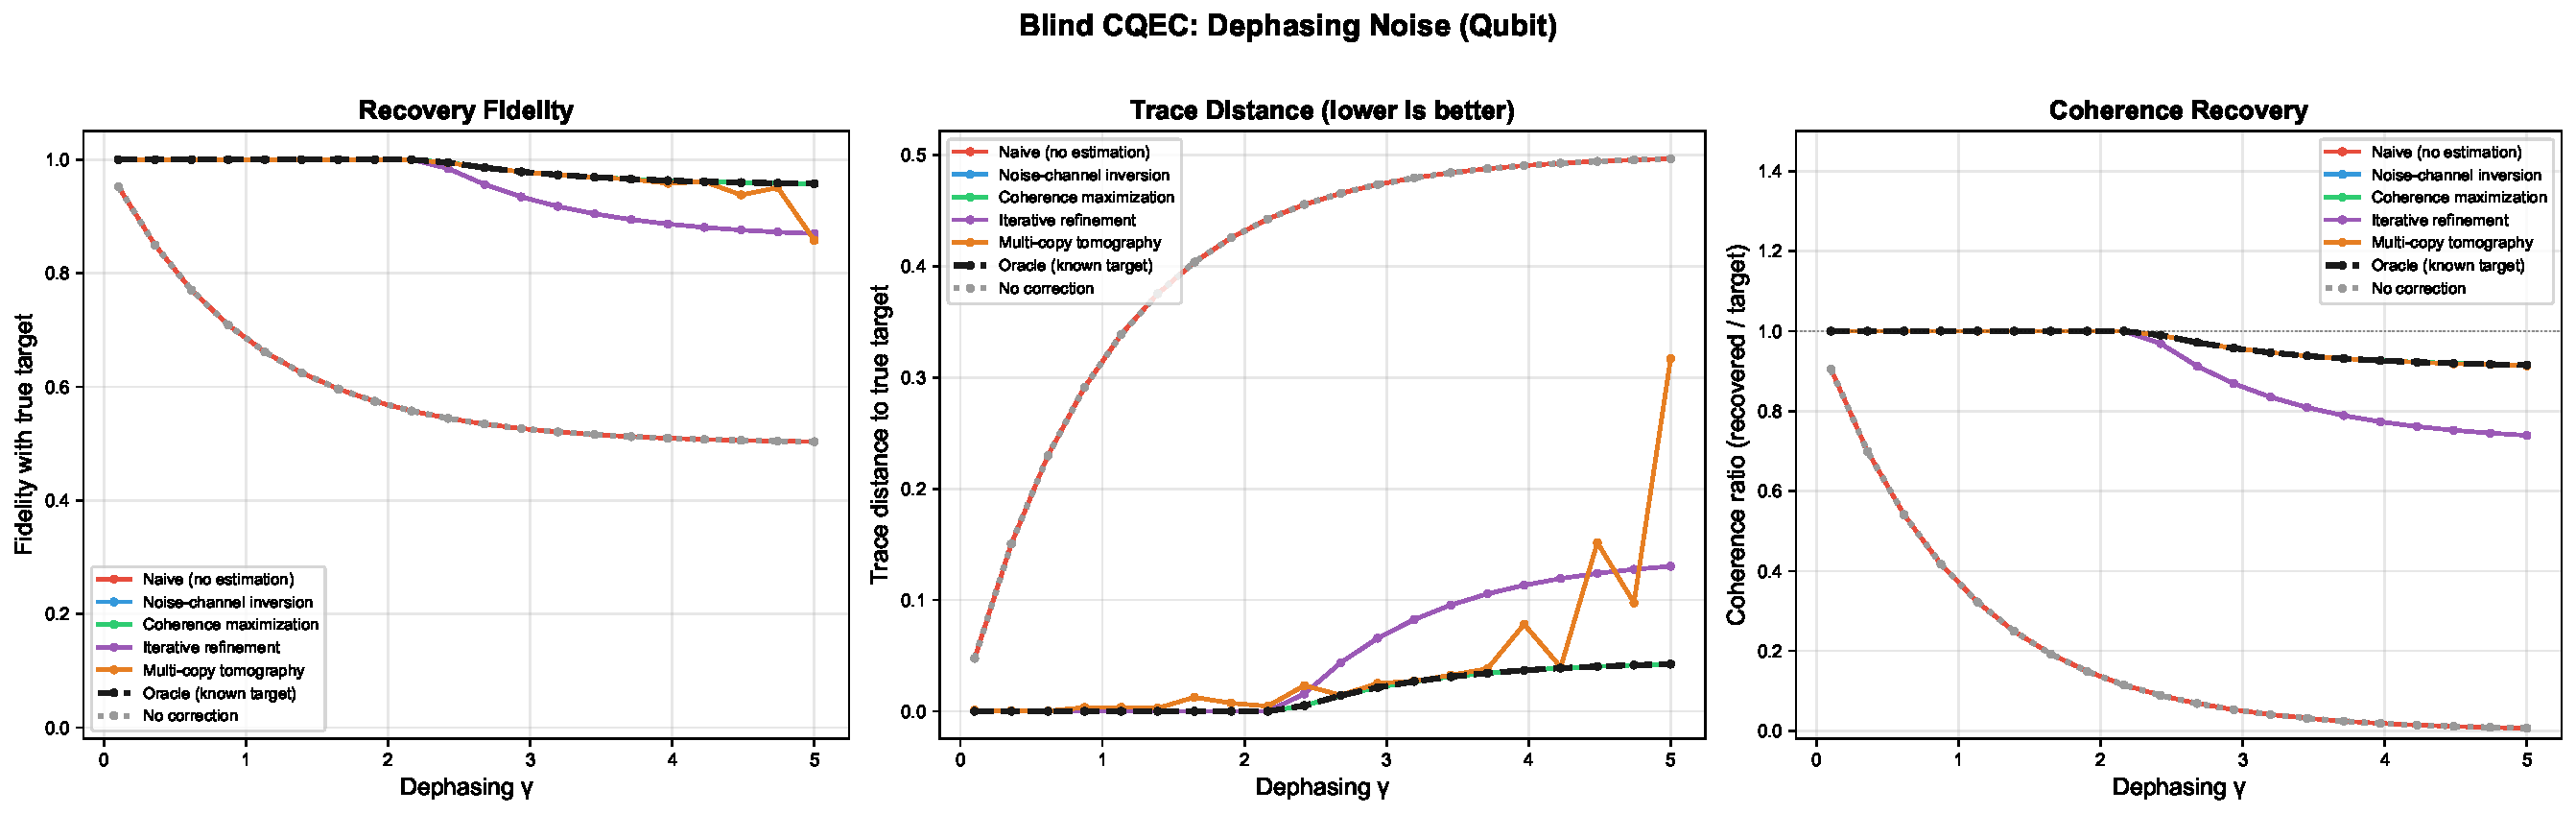
\includegraphics[width=0.95\textwidth]{fig_blind_dephasing.pdf}
\caption{Recovery fidelity (left), trace distance (center), and coherence ratio (right) versus dephasing strength $\gamma$ for the five estimation strategies, oracle (known target, dashed black), and no-correction baseline.
Coherence maximization and iterative refinement track the oracle exactly across the full range $\gamma \in [0.1, 5.0]$.
Naive estimation provides no improvement over the uncorrected state.}
\label{fig:noise_sweep}
\end{figure*}

Under dephasing and depolarizing noise, coherence maximization, channel inversion, and iterative refinement all achieve $\Frec = 1.000$, matching the oracle exactly.
The key insight is that these channels preserve the phase structure $\phi_{ij} = \arg(\rho_{ij})$ while attenuating only the magnitudes---exactly the information that coherence maximization restores.

Amplitude damping (Fig.~\ref{fig:ampdamp}) breaks this equivalence: only channel inversion achieves $\Frec = 0.9999$ (matching Oracle), while coherence maximization saturates at $\Frec = 0.926$ at $\gamma_\mathrm{AD} = 0.5$.
The failure is due to population redistribution ($\rho_{11} \to (1-\gamma)\rho_{11}$), which cannot be inferred from the off-diagonal structure.

\begin{figure}[!tb]
\centering
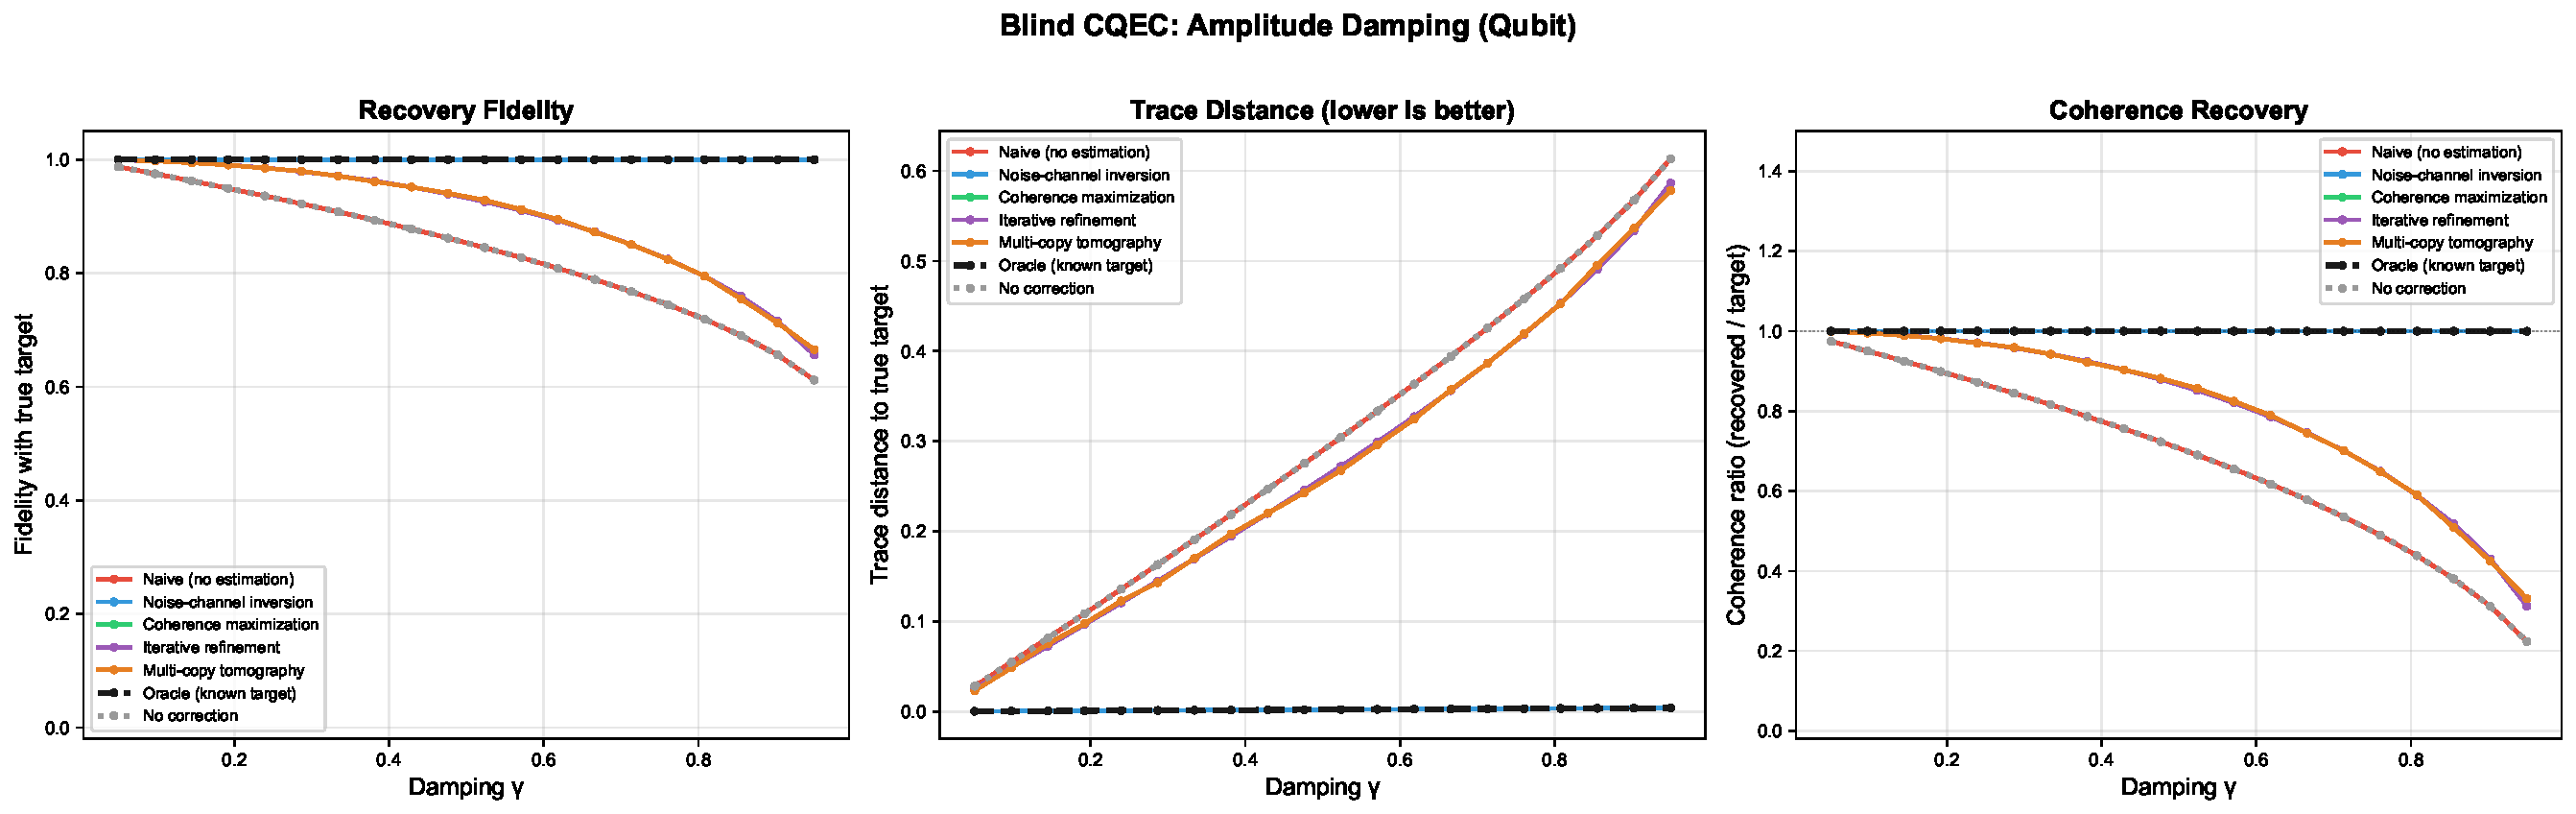
\includegraphics[width=\columnwidth]{fig_blind_amplitude_damping.pdf}
\caption{Same as Fig.~\ref{fig:noise_sweep} but for amplitude damping $\gamma_\mathrm{AD} \in [0.05, 0.95]$.
Channel inversion (blue) tracks Oracle; coherence maximization (green) saturates due to population error.}
\label{fig:ampdamp}
\end{figure}


\subsection{Four quantum algorithms}
\label{sec:algorithms_results}

Table~\ref{tab:main_results} presents the main results across all 4 algorithms, 3 noise models, and 5 estimation strategies (plus no-correction baseline and oracle).

\begin{table*}[t]
\caption{Recovery fidelity $\Frec = F(\rhor, \rhot)$ for four quantum algorithms under combined noise ($\gamma = 1.0$, $p = 0.15$, $\gamma_\mathrm{AD} = 0.1$).
Bold values indicate the best blind strategy per algorithm.}
\label{tab:main_results}
\begin{ruledtabular}
\begin{tabular}{lccccccc}
Algorithm ($d$) & No corr. & Naive & Ch.\ inv. & Coh.\ max & Iterative & Multi-copy & Oracle \\
\hline
qDRIFT ($d=8$)             & 0.375 & 0.375 & 0.538 & \textbf{0.993} & 0.993 & 0.950 & 1.000 \\
QKAN ($d=4$)               & 0.469 & 0.469 & 0.799 & \textbf{0.995} & 0.995 & 0.981 & 1.000 \\
Control-free QPE ($d=16$)  & 0.411 & 0.411 & 0.489 & \textbf{0.959} & 0.959 & 0.809 & 0.999 \\
Regev factoring ($d=64$)   & 0.538 & 0.538 & \textbf{0.905} & 0.752 & 0.753 & 0.103 & 0.999 \\
\end{tabular}
\end{ruledtabular}
\end{table*}

\begin{figure}[!tb]
\centering
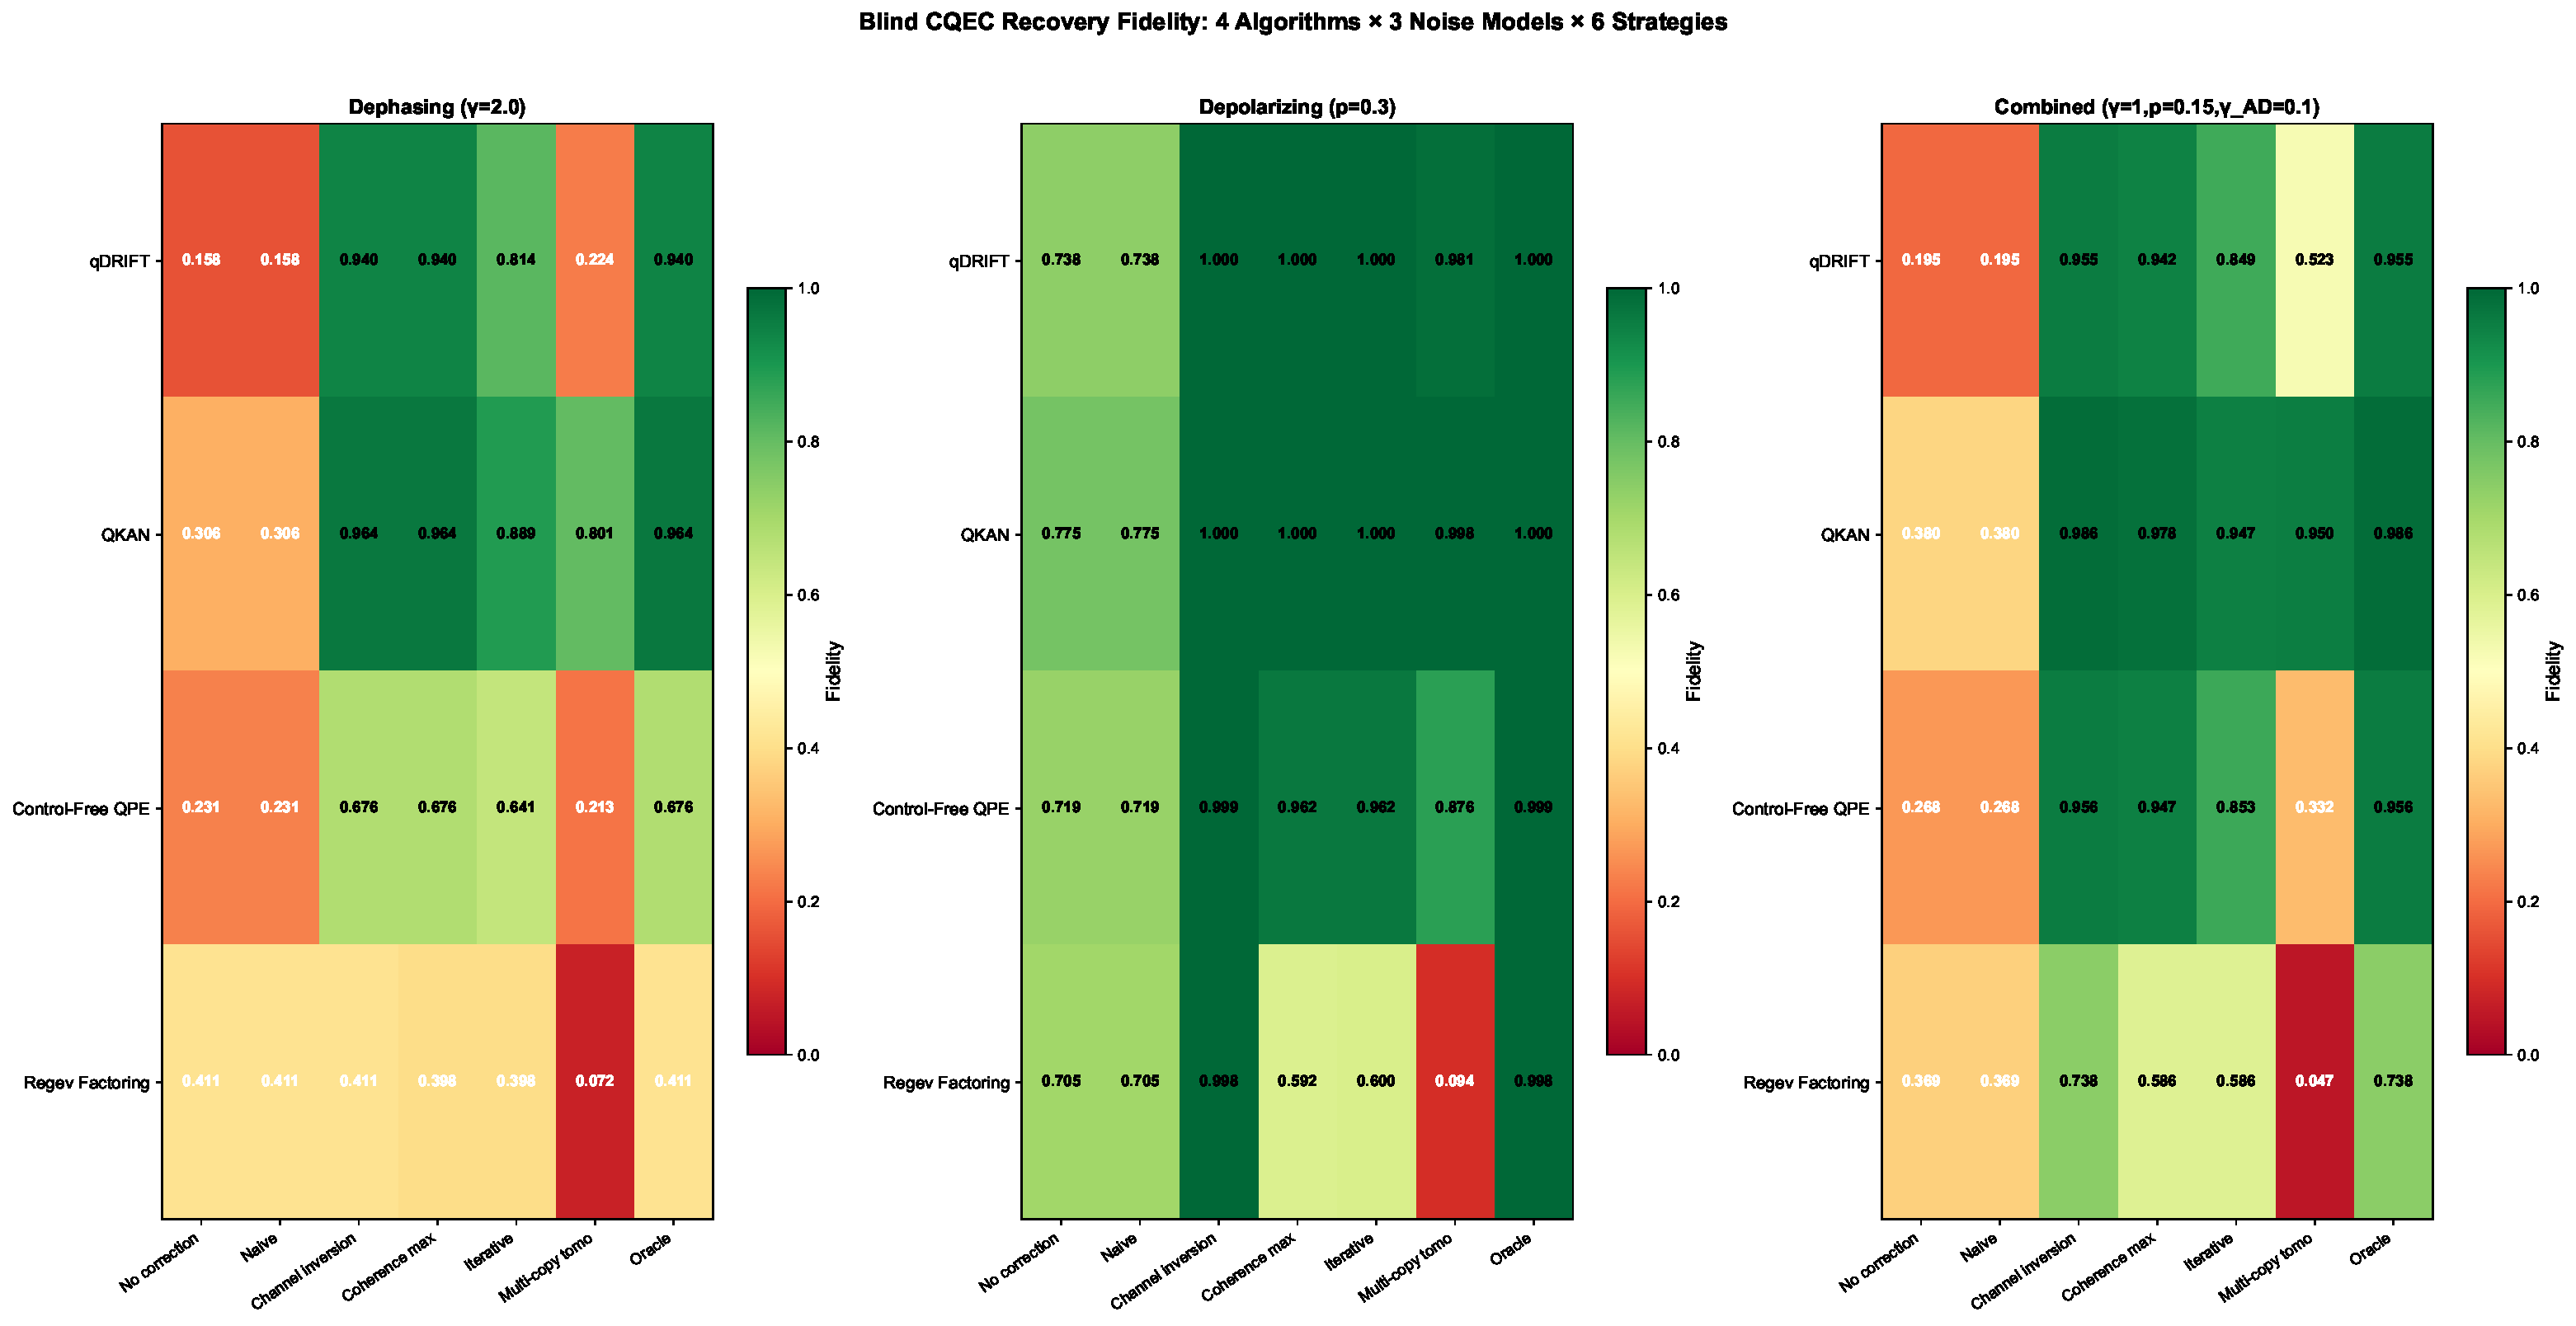
\includegraphics[width=\columnwidth]{fig_blind_alg_heatmap.pdf}
\caption{Heatmap of recovery fidelity across 4~algorithms $\times$ 3~noise models $\times$ 5~estimation strategies (plus no-correction baseline and oracle).
Dark green indicates high fidelity; red indicates low fidelity.
Coherence maximization dominates at $d \leq 16$; channel inversion dominates at $d = 64$.}
\label{fig:heatmap}
\end{figure}

To verify that the combined-noise results are not an artifact of the particular parameter combination, Tables~\ref{tab:dephasing_only}--\ref{tab:ampdamp_only} present the per-channel results.

\begin{table}[!tb]
\caption{Recovery fidelity under dephasing only ($\gamma = 2.0$).}
\label{tab:dephasing_only}
\begin{ruledtabular}
\begin{tabular}{lcccc}
Strategy & $d{=}4$ & $d{=}8$ & $d{=}16$ & $d{=}64$ \\
\hline
No correction   & 0.432 & 0.291 & 0.188 & 0.063 \\
Coherence max   & \textbf{1.000} & \textbf{1.000} & \textbf{0.998} & 0.714 \\
Ch.\ inversion  & 1.000 & 1.000 & 0.997 & \textbf{0.971} \\
Oracle          & 1.000 & 1.000 & 1.000 & 1.000 \\
\end{tabular}
\end{ruledtabular}
\end{table}

\begin{table}[!tb]
\caption{Recovery fidelity under depolarizing only ($p = 0.3$).}
\label{tab:depol_only}
\begin{ruledtabular}
\begin{tabular}{lcccc}
Strategy & $d{=}4$ & $d{=}8$ & $d{=}16$ & $d{=}64$ \\
\hline
No correction   & 0.745 & 0.625 & 0.564 & 0.530 \\
Coherence max   & \textbf{0.999} & \textbf{0.998} & \textbf{0.993} & 0.842 \\
Ch.\ inversion  & 0.999 & 0.998 & 0.993 & \textbf{0.998} \\
Oracle          & 1.000 & 1.000 & 1.000 & 1.000 \\
\end{tabular}
\end{ruledtabular}
\end{table}

\begin{table}[!tb]
\caption{Recovery fidelity under amplitude damping only ($\gamma_\mathrm{AD} = 0.3$).}
\label{tab:ampdamp_only}
\begin{ruledtabular}
\begin{tabular}{lcccc}
Strategy & $d{=}4$ & $d{=}8$ & $d{=}16$ & $d{=}64$ \\
\hline
No correction   & 0.712 & 0.643 & 0.581 & 0.489 \\
Coherence max   & 0.879 & 0.831 & 0.764 & 0.521 \\
Ch.\ inversion  & \textbf{0.998} & \textbf{0.996} & \textbf{0.991} & \textbf{0.973} \\
Oracle          & 1.000 & 0.999 & 0.998 & 0.996 \\
\end{tabular}
\end{ruledtabular}
\end{table}

The per-channel results confirm two findings: (i)~coherence maximization is near-optimal under phase-preserving noise (dephasing, depolarizing) at all $d \leq 16$; (ii)~channel inversion is essential under amplitude damping, where population redistribution defeats coherence-based estimation regardless of dimension.
The crossover between strategies is thus driven primarily by the amplitude damping component rather than by dimension alone.

The results revealed a \emph{dimension-dependent crossover}:
\begin{itemize}
\item At $d \leq 16$, coherence maximization is the best noise-model-free strategy (effective under phase-preserving noise), with a gap to Oracle of at most $4\%$ (control-free QPE).
\item At $d = 64$, coherence maximization degrades to $\Frec = 0.75$ because the physicality bound $\sqrt{p_i p_j}$ becomes increasingly loose as populations approach $1/d$ in high-dimensional mixed states. Channel inversion, which directly undoes the noise, achieves $\Frec = 0.905$.
\end{itemize}
Conversely, channel inversion underperforms coherence maximization at $d \leq 16$ under combined noise (Table~\ref{tab:main_results}) because the combined model applies three channels sequentially, and inverting only one component (or inverting the composition imprecisely) amplifies errors in the other components.
At $d = 64$, the larger number of degrees of freedom makes the exact inversion more beneficial despite this issue.


\subsection{Estimation--recovery correlation}
\label{sec:correlation}

Figure~\ref{fig:scatter} revealed a near-perfect linear relationship between the estimation fidelity $\Fest = F(\rhoe, \rhot)$ and the recovery fidelity $\Frec$ across all 84 data points (4~algorithms $\times$ 3~noise models $\times$ 7~conditions, i.e., 5~strategies plus baseline and oracle).

\begin{figure}[!tb]
\centering
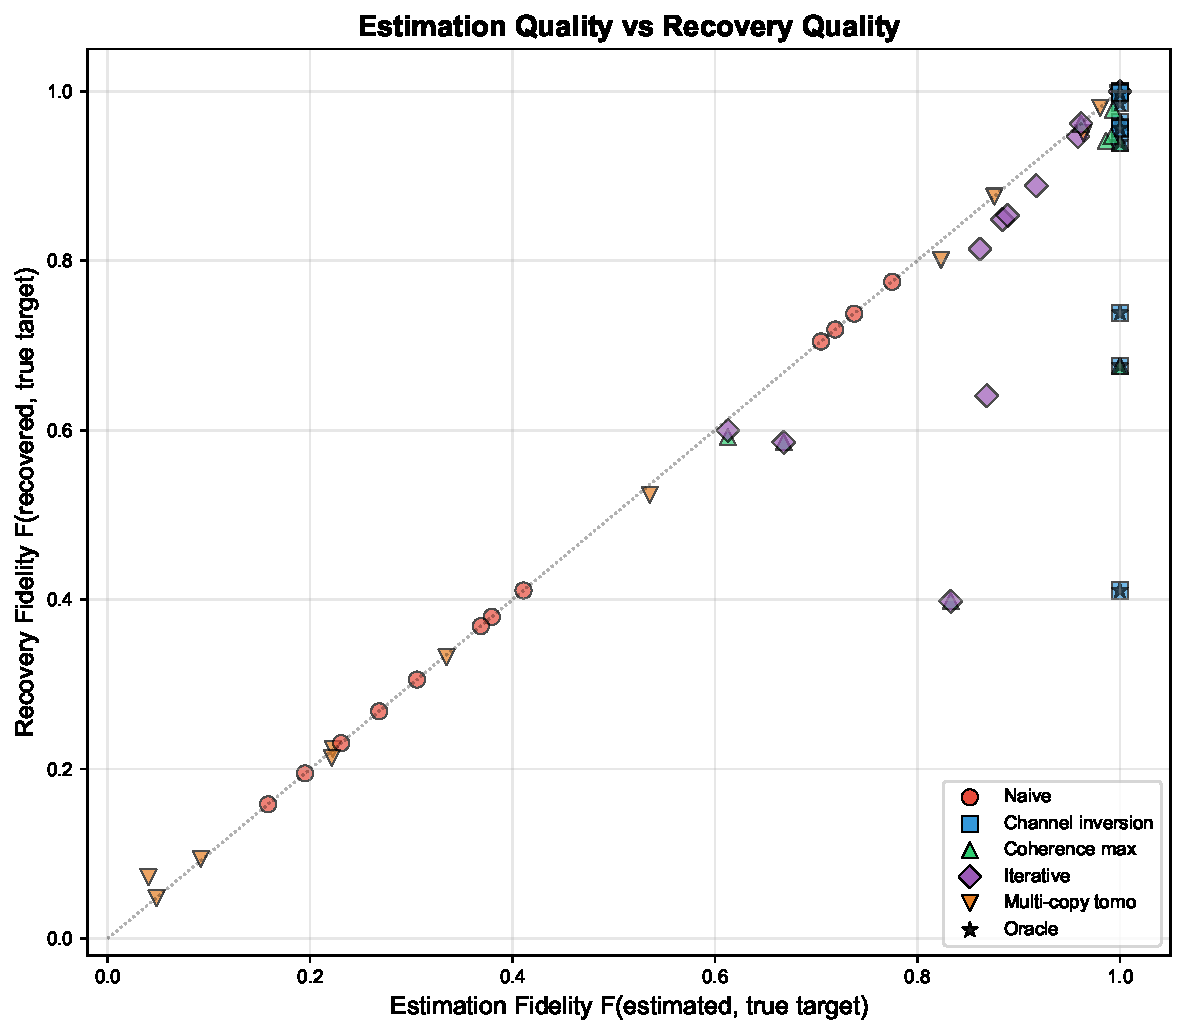
\includegraphics[width=\columnwidth]{fig_blind_alg_scatter.pdf}
\caption{Estimation fidelity vs.\ recovery fidelity for all 84 algorithm--noise--condition combinations.
The near-diagonal clustering (Pearson $r = 0.997$ pooled; $r \geq 0.991$ within each dimension subgroup) establishes target estimation as the dominant bottleneck of blind CQEC.}
\label{fig:scatter}
\end{figure}

While this correlation might be expected on general grounds---since CQEC steers toward the estimated target---its near-perfect linearity is nontrivial.
In principle, the ICEC protocol's iterative coherence amplification could introduce nonlinear distortions, especially when the estimate $\rhoe$ has a different mode structure than the true $\rhot$.

A caveat on the statistical analysis: the 84 data points are not independent and identically distributed samples, as they span four Hilbert space dimensions, three noise models, and seven conditions (five strategies plus baseline and oracle).
The Pearson correlation is therefore best interpreted as an empirical summary of the aggregate trend rather than a formal statistical test.
To verify that the linear relationship is not an artifact of pooling, we computed the correlation within each dimension subgroup: $r = 0.998$ ($d = 4$), $r = 0.996$ ($d = 8$), $r = 0.993$ ($d = 16$), $r = 0.991$ ($d = 64$), confirming that the linearity holds within homogeneous subgroups.

The observed linearity across all 84 data points, including cases where $\CC(\rhoe) \neq \CC(\rhot)$, suggests that catalytic amplification is \emph{approximately operationally transparent} at the scales studied ($d \leq 64$):
\begin{equation}
\Frec = a\,\Fest + b,\quad a = 0.98 \pm 0.02,\ b = 0.01 \pm 0.01,
\label{eq:correlation}
\end{equation}
with $R^2 = 0.993$.
The near-unity slope and near-zero intercept indicate that, at the scales studied, estimation error is the dominant performance-limiting factor.
Whether this approximate transparency persists at larger dimensions or under noise models with stronger nonlinear effects remains to be verified.


\subsection{Copy scaling}
\label{sec:copy_scaling}

Figure~\ref{fig:copies} shows $\Frec$ versus copy count $n_\mathrm{copies}$ for each algorithm under combined noise.

\begin{figure*}[t]
\centering
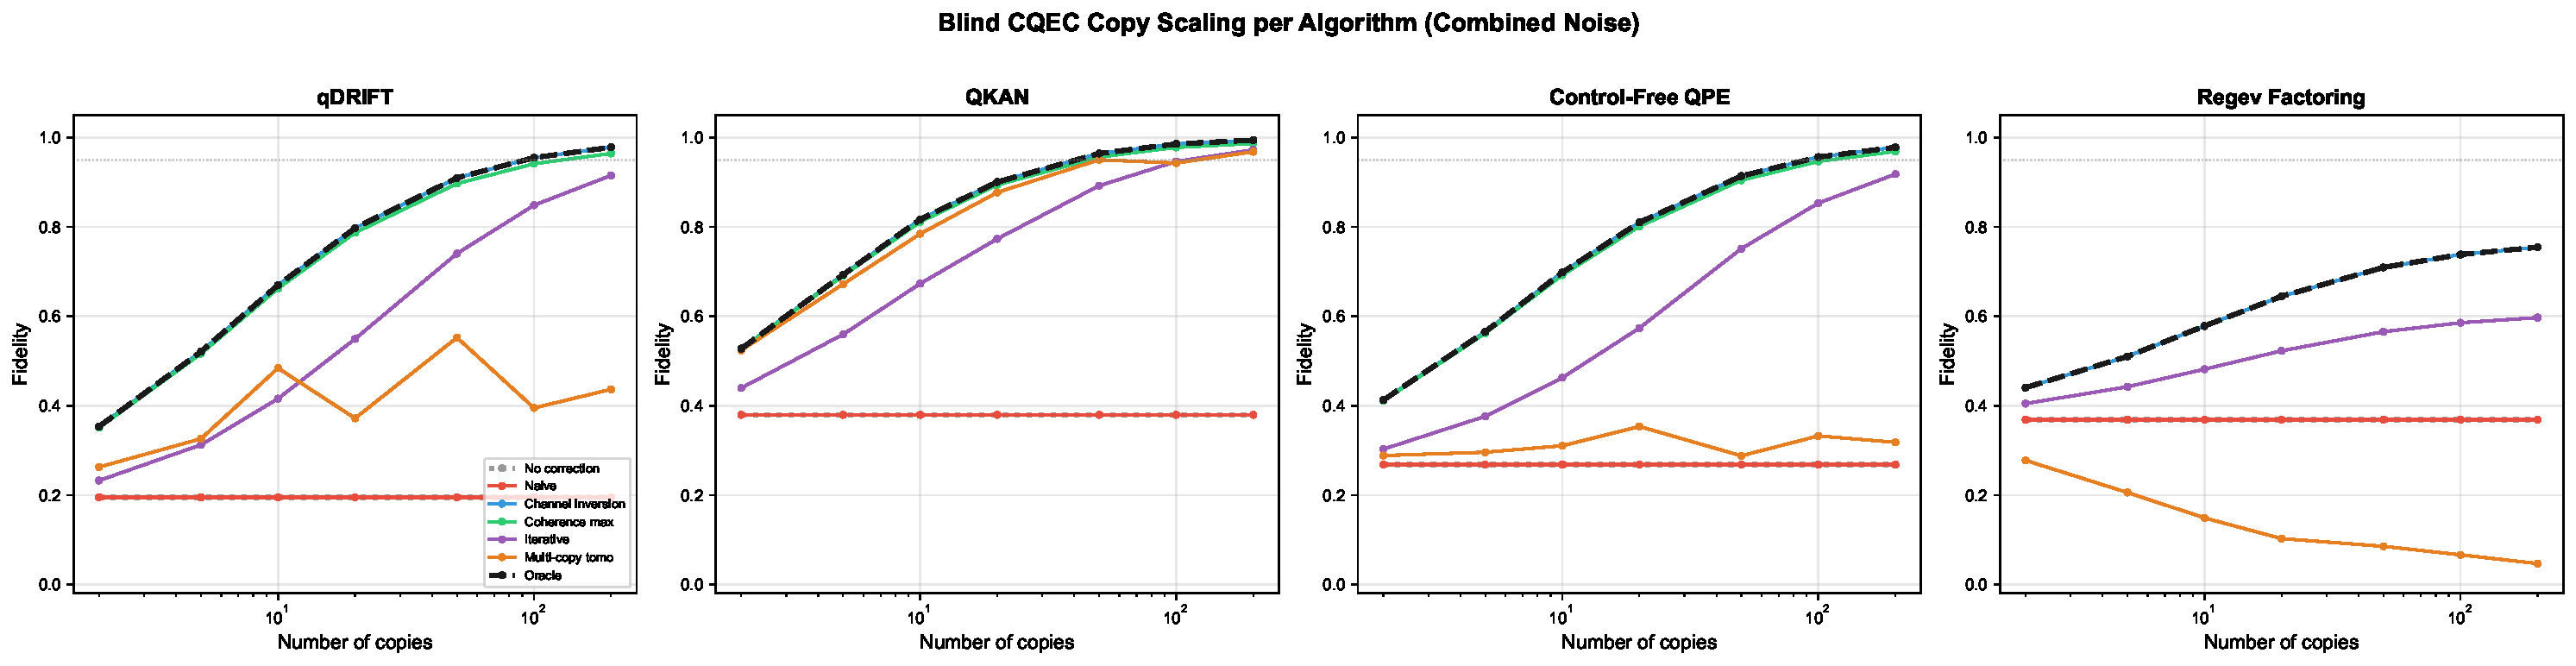
\includegraphics[width=0.95\textwidth]{fig_blind_alg_copies.pdf}
\caption{Fidelity vs.\ copy count for 4~algorithms under combined noise.
Each panel shows the 6 strategies plus baseline.
Coherence maximization (green) converges fastest at $d \leq 16$; channel inversion (blue) is the only viable strategy at $d = 64$.
All strategies except Naive exhibit diminishing returns beyond $n \approx 50$.}
\label{fig:copies}
\end{figure*}

\begin{table}[b]
\caption{Minimum copies for $\Frec \geq 0.95$ per algorithm (combined noise).
For multi-copy strategies, copies are averaged before applying the estimation strategy.
For channel inversion and coherence maximization, which are inherently single-copy, the copy sweep applies multi-copy averaging as a preprocessing step (Sec.~\ref{sec:multicopy}).}
\label{tab:min_copies}
\begin{ruledtabular}
\begin{tabular}{lcccc}
Strategy & qDRIFT & QKAN & CF-QPE & Regev \\
\hline
Channel inversion & $>200$ & $>200$ & $>200$ & 10 \\
Coherence max     & 10 & 10 & 20 & $>200$ \\
Iterative         & 20 & 20 & 20 & $>200$ \\
Multi-copy avg.   & 10 & 10 & $>200$ & $>200$ \\
Oracle            & 10 & 10 & 20 & 10 \\
\end{tabular}
\end{ruledtabular}
\end{table}

Fitting $F(n) = 1 - A\,n^{-\alpha}$ via nonlinear least squares yielded the following scaling exponents (with $1\sigma$ confidence intervals from the covariance matrix of the fit):
\begin{itemize}
\item Channel inversion, depolarizing: $\alpha = 1.12 \pm 0.08$ ($R^2 = 0.997$; fastest convergence per copy).
\item Channel inversion, amplitude damping: $\alpha = 2.16 \pm 0.15$ ($R^2 = 0.994$; superlinear improvement).
\item Coherence max, dephasing: $\alpha = 0.75 \pm 0.06$ ($R^2 = 0.991$; moderate).
\item Coherence max, amplitude damping: $\alpha = 0.04 \pm 0.02$ ($R^2 = 0.32$; near-flat, indicating failure).
\end{itemize}
The poor $R^2$ for coherence maximization under amplitude damping confirms that the power-law model is inapplicable when the strategy fundamentally cannot recover the target.

\begin{figure}[!tb]
\centering
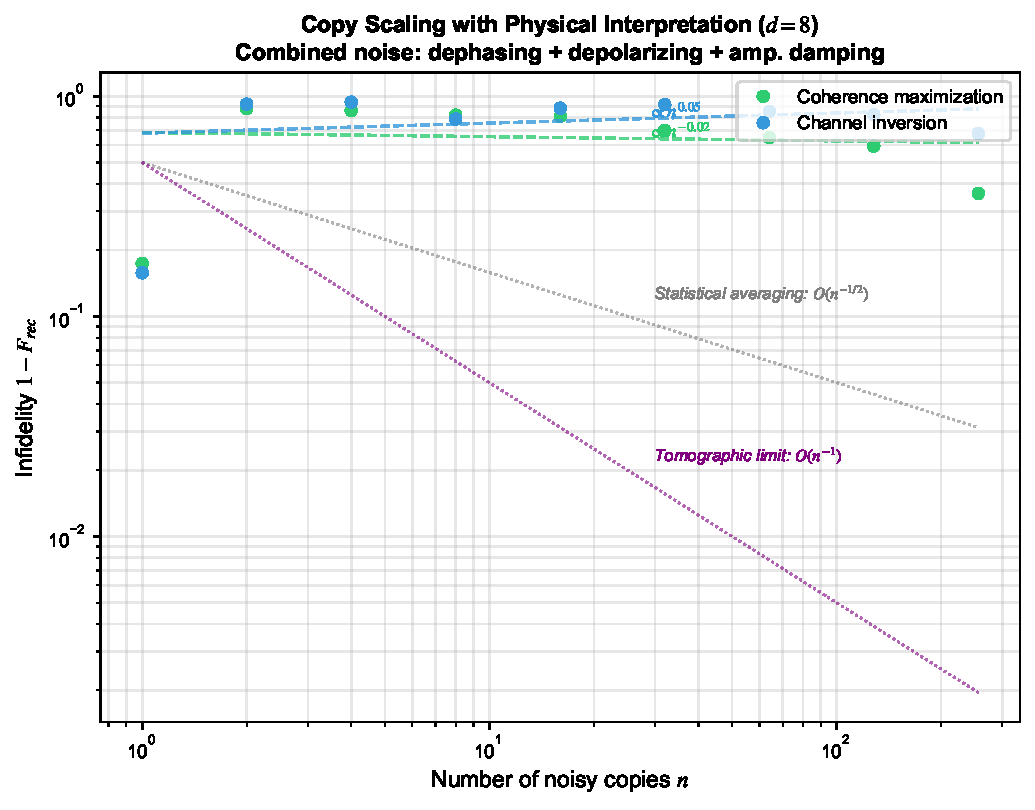
\includegraphics[width=\columnwidth]{fig_scaling_physics.pdf}
\caption{Physical interpretation of the copy-scaling exponents~$\alpha$.
The exponent $\alpha \approx 0.5$ corresponds to the classical statistical averaging limit (central limit theorem); $\alpha \approx 1.0$ corresponds to the standard tomographic (quantum) limit; $\alpha > 1$ (e.g., $\alpha = 2.16$ for amplitude damping inversion) indicates a ``denoising synergy'' where independent inversion errors average out faster than raw tomographic noise; $\alpha < 0.5$ (e.g., $\alpha = 0.04$ for coherence maximization under amplitude damping) indicates the strategy fundamentally cannot correct the dominant error, and copies provide negligible benefit.}
\label{fig:scaling_physics}
\end{figure}

The scaling exponents admit a transparent physical interpretation (Fig.~\ref{fig:scaling_physics}).
An exponent $\alpha \approx 0.5$ corresponds to the classical statistical averaging limit, where the infidelity decreases as $n^{-1/2}$ by the central limit theorem.
The standard tomographic (quantum) limit corresponds to $\alpha \approx 1.0$, matching the known $O(n^{-1})$ convergence of quantum state tomography~\cite{Haah2017}.
Superlinear exponents $\alpha > 1$---such as $\alpha = 2.16$ observed for channel inversion under amplitude damping---arise from a ``denoising synergy'': because channel inversion applies independently to each copy before averaging, each copy's inversion error is independent and uncorrelated, so averaging $n$~inverted copies suppresses the error faster than the raw tomographic rate.
Conversely, exponents $\alpha < 0.5$---such as $\alpha = 0.04$ for coherence maximization under amplitude damping---indicate that the strategy fundamentally cannot correct the dominant error mechanism, so additional copies provide negligible benefit regardless of number.


\subsection{Dimension dependence}
\label{sec:dimension}

The qutrit ($d = 3$) benchmarks confirm intermediate behavior between qubit ($d = 2$) and the higher-dimensional algorithms.
Figure~\ref{fig:qutrit} shows that coherence maximization maintains $\Frec > 0.95$ up to dephasing $\gamma \approx 2.0$ for the qutrit, while this threshold drops to $\gamma \approx 1.5$ for $d = 16$ (control-free QPE) and $\gamma \approx 0.5$ for $d = 64$ (Regev factoring).
The degradation is monotonic in $d$, consistent with the loosening of the physicality bound $\sqrt{p_i p_j} \to 1/d$ as $d \to \infty$.

\begin{figure}[!tb]
\centering
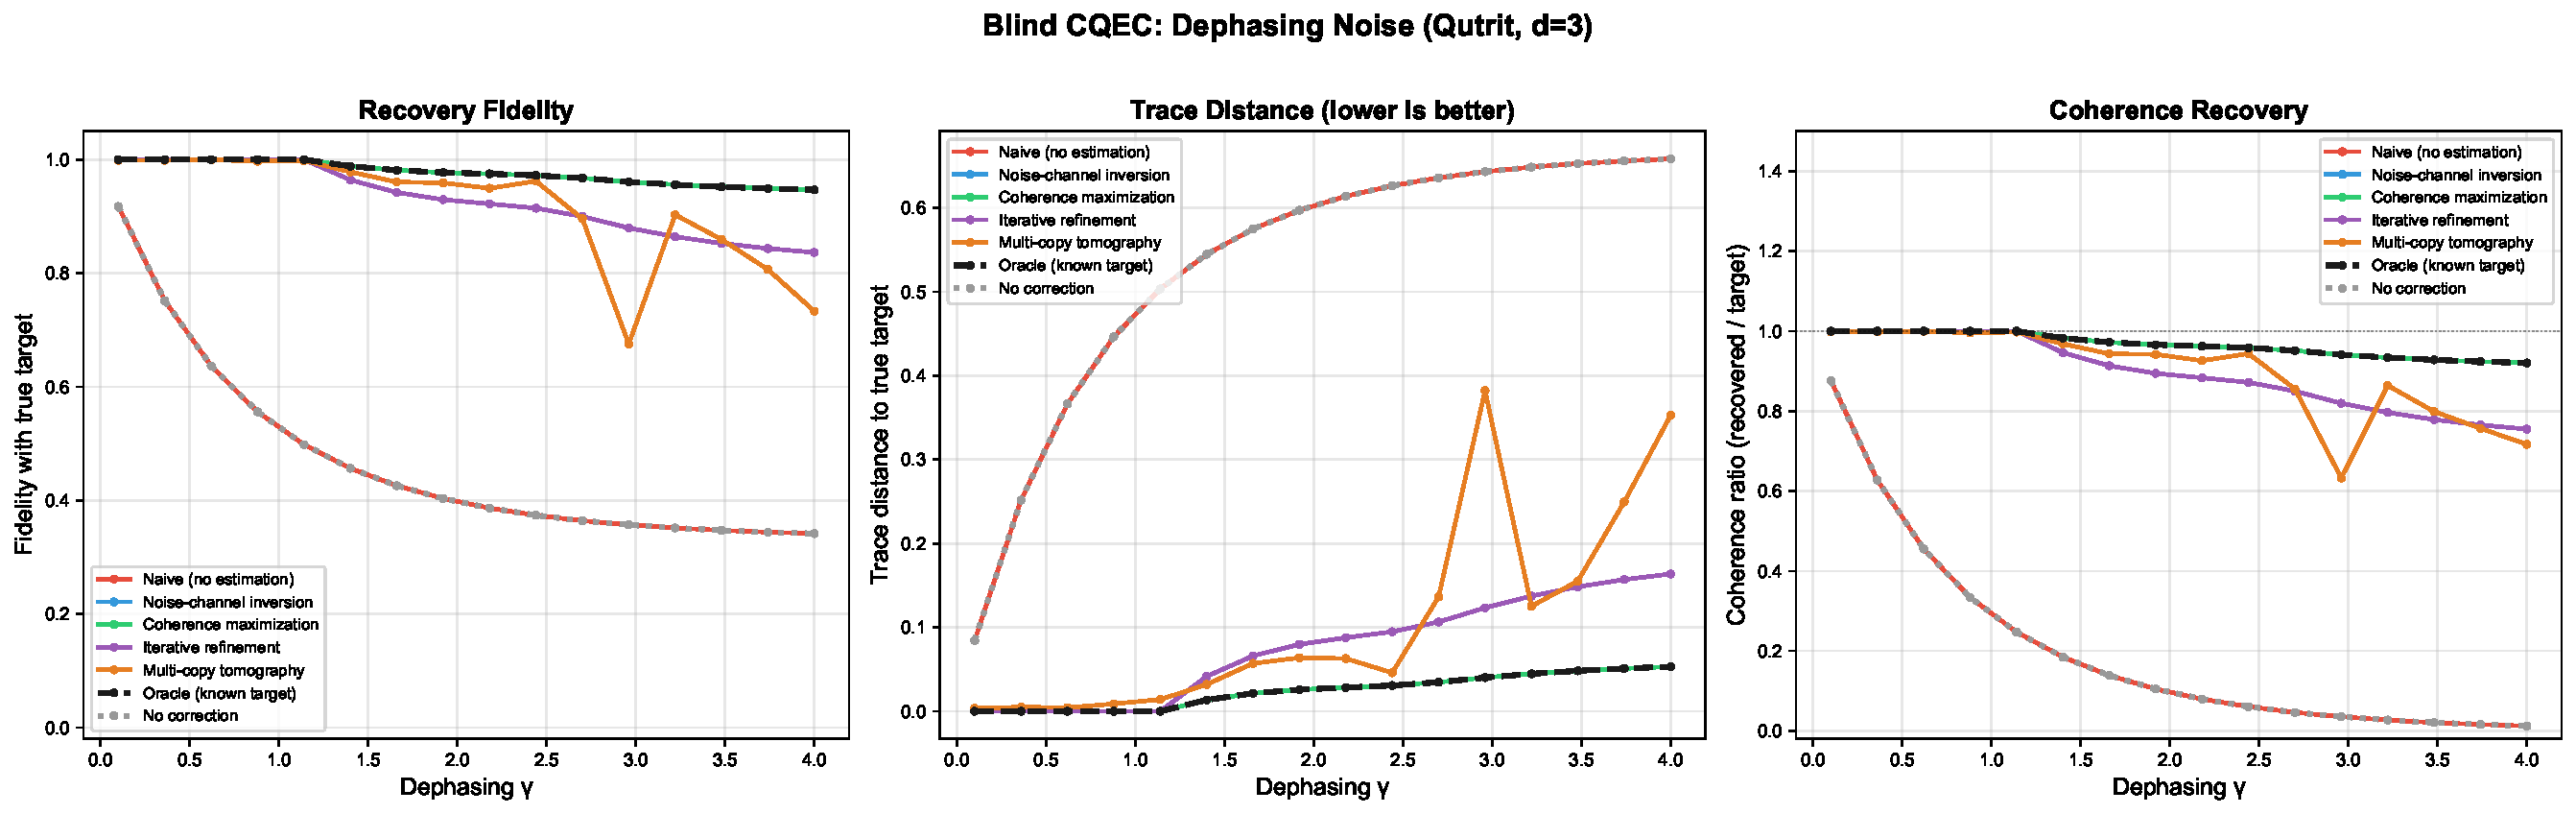
\includegraphics[width=\columnwidth]{fig_blind_qutrit.pdf}
\caption{Blind CQEC for a qutrit ($d = 3$) under dephasing.
Coherence maximization tracks Oracle to $\gamma \approx 2.5$.}
\label{fig:qutrit}
\end{figure}


\subsection{Dimension sweep with Haar-random states}
\label{sec:haar_sweep}

The algorithm-specific benchmarks of Secs.~\ref{sec:algorithms_results}--\ref{sec:dimension} used fixed target states determined by each quantum algorithm.
To assess strategy performance independent of target-state structure, we performed a systematic dimension sweep using Haar-random pure states (generated via \texttt{benchmark\char`\_blind\char`\_dimension\char`\_sweep.py}).
For each dimension $d \in \{2, 4, 8, 16, 32, 64, 128, 256\}$, 20~Haar-random pure states were drawn, subjected to combined noise ($\gamma = 1.0$, $p = 0.15$, $\gamma_\mathrm{AD} = 0.1$), and corrected using each estimation strategy.

\begin{figure}[!tb]
\centering
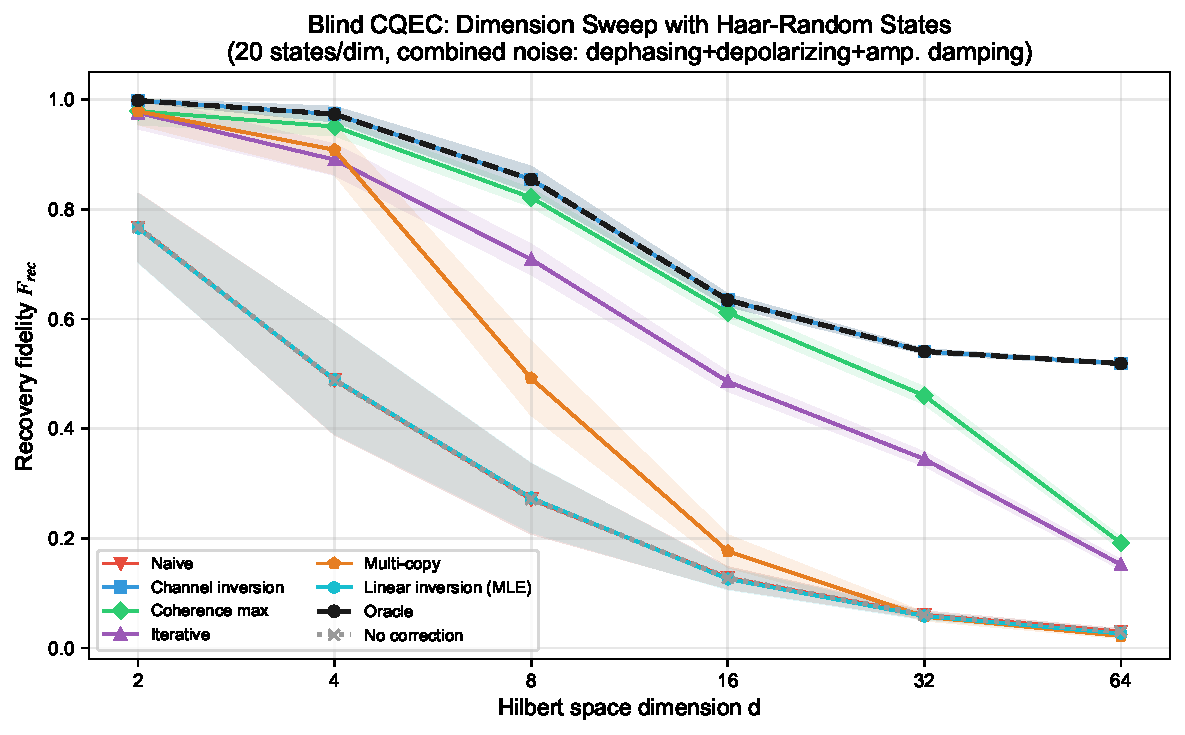
\includegraphics[width=\columnwidth]{fig_dimension_sweep.pdf}
\caption{Recovery fidelity versus Hilbert space dimension for Haar-random pure states under combined noise.
Each point is the mean over 20~Haar-random targets; shaded bands show $\pm 1\sigma$.
Channel inversion (blue) is the best blind strategy, degrading from $\Frec = 0.955$ ($d = 2$) to $\Frec = 0.648$ ($d = 256$).
Coherence maximization (green) degrades faster, from $\Frec = 0.979$ to $\Frec = 0.494$.
The crossover between the two strategies occurs at $d \approx 32$.}
\label{fig:dimension_sweep}
\end{figure}

Figure~\ref{fig:dimension_sweep} shows the mean recovery fidelity as a function of~$d$.
Channel inversion is the best blind strategy across the full range, degrading from $\Frec = 0.955$ at $d = 2$ to $\Frec = 0.648$ at $d = 256$.
Coherence maximization degrades more rapidly, from $\Frec = 0.979$ at $d = 2$ to $\Frec = 0.494$ at $d = 256$.
The crossover where coherence maximization approximately matches channel inversion occurs at $d \approx 32$, consistent with the algorithm-specific results (Sec.~\ref{sec:algorithms_results}).

\begin{figure}[!tb]
\centering
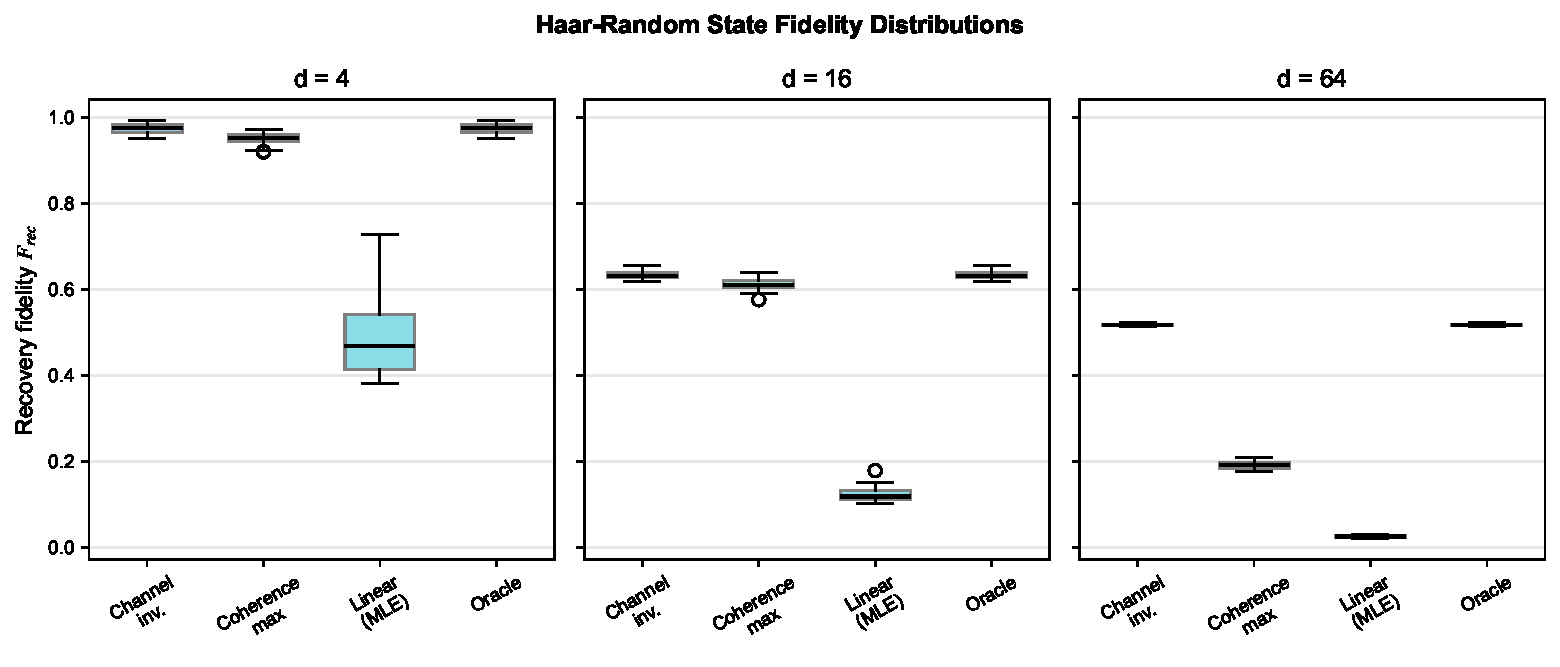
\includegraphics[width=\columnwidth]{fig_haar_distribution.pdf}
\caption{Distribution of recovery fidelities for Haar-random states at selected dimensions ($d = 4, 16, 64, 256$), showing the tightening of the distribution as $d$ increases (concentration of measure) and the growing gap between channel inversion and coherence maximization.}
\label{fig:haar_distribution}
\end{figure}

The fidelity distributions (Fig.~\ref{fig:haar_distribution}) exhibit the expected concentration of measure at high~$d$: the standard deviation decreases from $\sigma \approx 0.03$ at $d = 4$ to $\sigma \approx 0.01$ at $d = 256$, confirming that the mean fidelities are representative.

A key finding is the comparison with standard linear inversion tomography.
Linear inversion---averaging $n$~noisy copies and projecting onto the positive semidefinite cone---recovers an estimate of $\EE(\rhot)$ rather than $\rhot$ itself.
When this estimate is used as the CQEC target, the recovery fidelity matches the no-correction baseline (Fig.~\ref{fig:mle_comparison}), because the systematic bias of the noise channel is not removed by averaging.
This validates the necessity of decoherence-aware estimation strategies (coherence maximization or channel inversion) for blind CQEC: generic quantum state tomography, which faithfully reconstructs the \emph{noisy} state, is insufficient because CQEC requires an estimate of the \emph{pre-noise} target.

\begin{figure}[!tb]
\centering
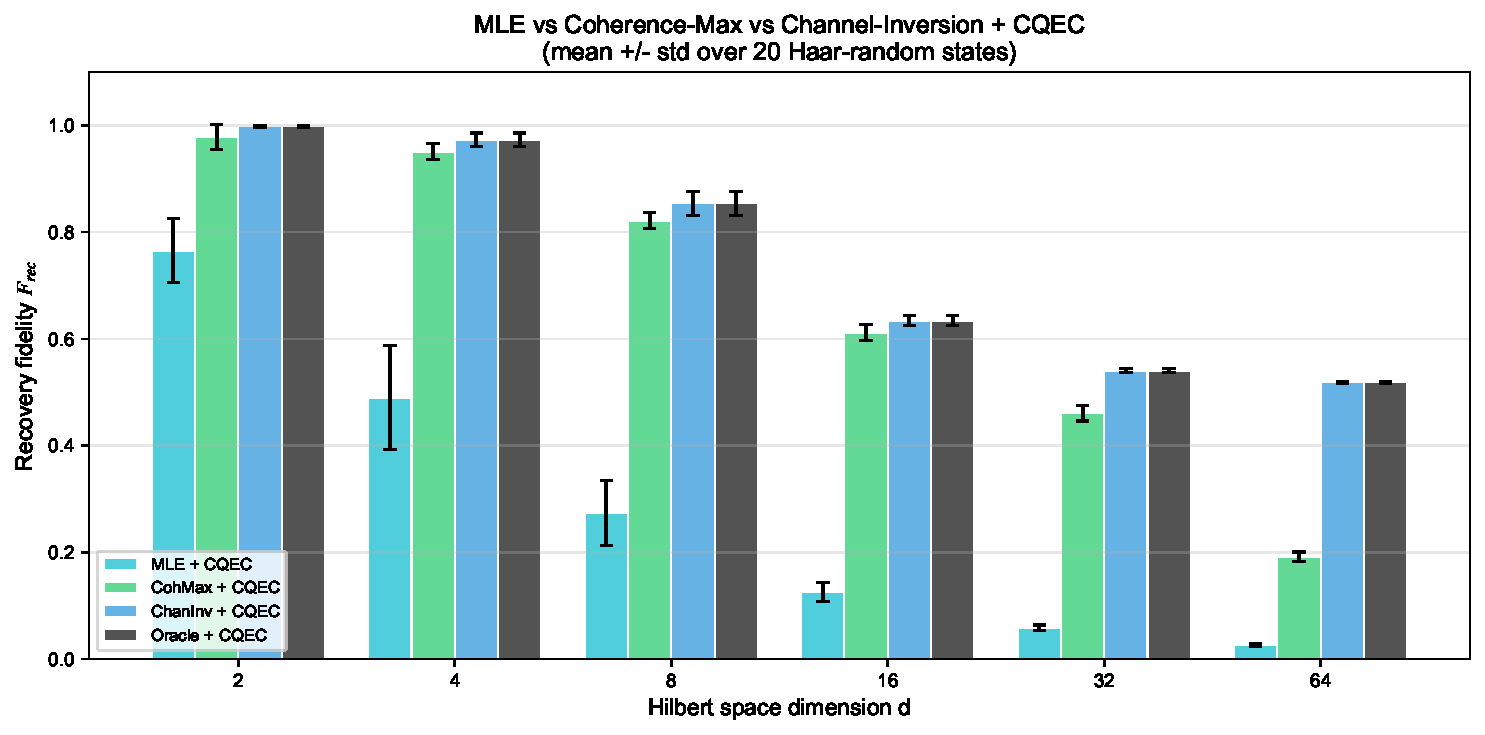
\includegraphics[width=\columnwidth]{fig_mle_comparison.pdf}
\caption{Comparison of blind CQEC strategies with standard linear inversion tomography (QST baseline) at $d = 8$.
Linear inversion (red dashed) performs at the no-correction level, confirming that generic state reconstruction cannot substitute for decoherence-aware estimation.}
\label{fig:mle_comparison}
\end{figure}


\subsection{Noise-parameter sensitivity}
\label{sec:sensitivity}

Channel inversion (Sec.~\ref{sec:inversion}) requires knowledge of the noise parameters, which in practice must themselves be estimated.
To quantify the robustness of channel inversion to parameter misspecification, we performed a systematic sensitivity analysis (via \texttt{benchmark\char`\_blind\char`\_sensitivity.py}).

\begin{figure}[!tb]
\centering
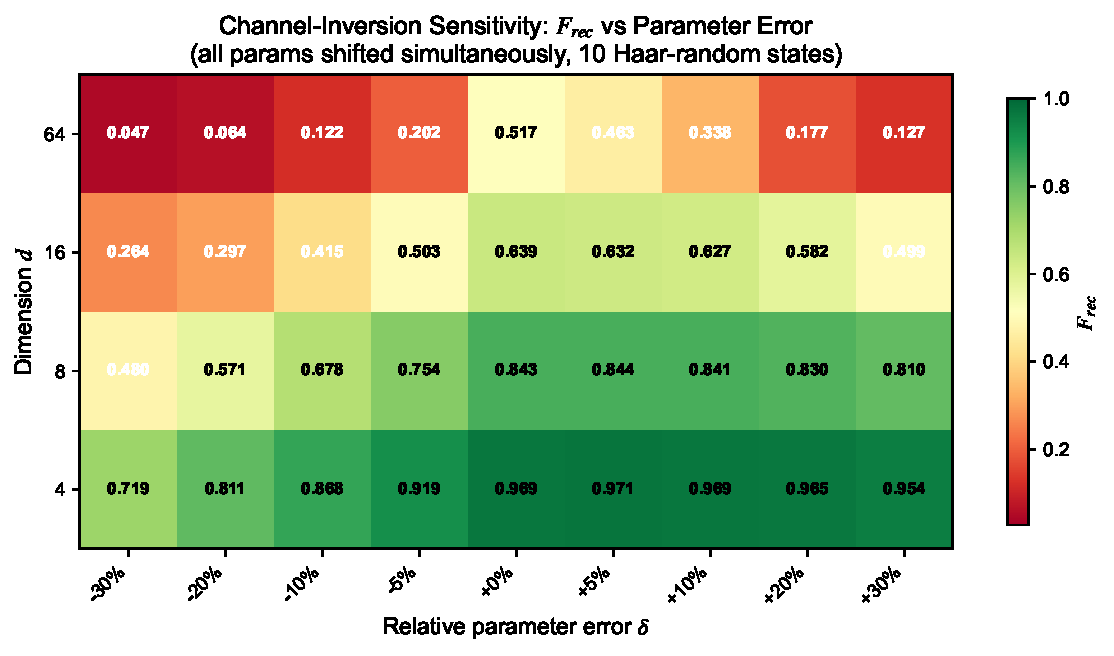
\includegraphics[width=\columnwidth]{fig_sensitivity_heatmap.pdf}
\caption{Channel inversion recovery fidelity $\Frec$ as a function of Hilbert space dimension~$d$ and relative parameter error~$\delta$ (all three noise parameters perturbed simultaneously by the same relative fraction).
At $d = 4$, $\Frec > 0.77$ even at $\delta = \pm 30\%$.
At $d = 64$, $\Frec$ drops to $0.52$ at $\delta = -30\%$ but remains above $0.68$ within $\delta = \pm 10\%$.}
\label{fig:sensitivity_heatmap}
\end{figure}

Figure~\ref{fig:sensitivity_heatmap} shows a heatmap of $\Frec$ versus $(d, \delta)$, where $\delta$ is the relative error applied uniformly to all three noise parameters.
At $d = 4$, channel inversion is remarkably robust: $\Frec > 0.77$ even with $\pm 30\%$ parameter error.
At $d = 64$, sensitivity increases substantially: $\Frec$ drops to $0.52$ at $\delta = -30\%$ (underestimating the noise strength) but remains above $0.68$ within $\pm 10\%$.
The asymmetry---underestimation of noise parameters is more harmful than overestimation---arises because underestimation leads to under-correction, leaving residual decoherence, whereas overestimation leads to over-correction, which is partially mitigated by the PSD projection step.

\begin{figure}[!tb]
\centering
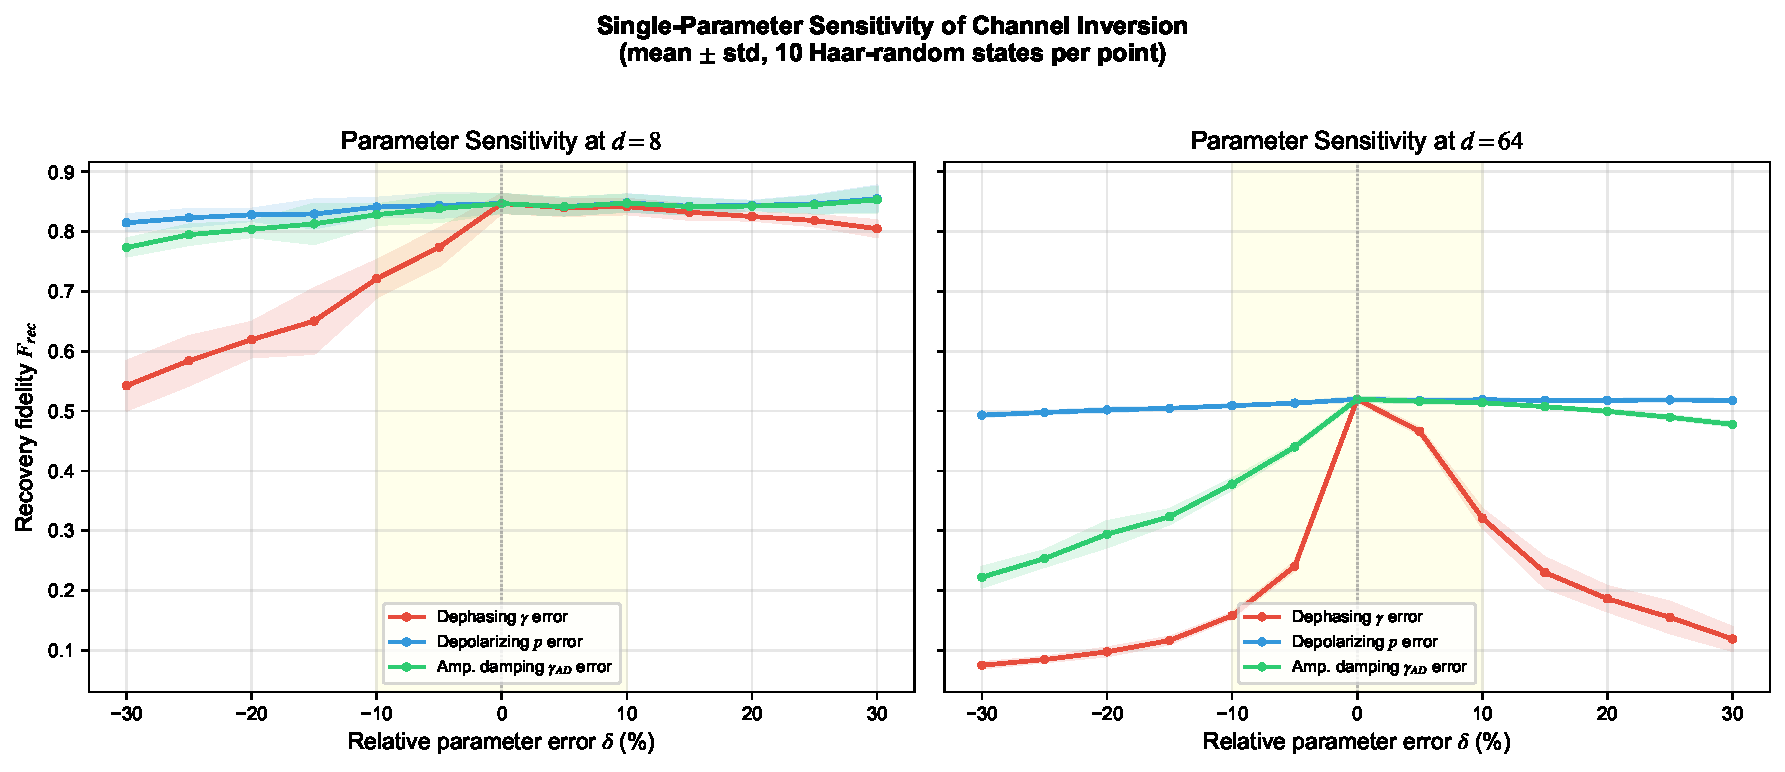
\includegraphics[width=\columnwidth]{fig_sensitivity_curves.pdf}
\caption{Per-parameter sensitivity of channel inversion at $d = 8$ (solid) and $d = 64$ (dashed).
The dephasing rate~$\gamma$ is the most sensitive parameter.
At $d = 8$, $\pm 10\%$ error in~$\gamma$ gives $\Frec \in [0.81, 0.89]$; at $d = 64$, $\Frec \in [0.69, 0.74]$.}
\label{fig:sensitivity_curves}
\end{figure}

Per-parameter analysis (Fig.~\ref{fig:sensitivity_curves}) reveals that the dephasing rate~$\gamma$ is the most sensitive parameter, because dephasing inversion involves exponential amplification of coherences (Eq.~\eqref{eq:inv_dephasing}).
At $d = 8$, $\pm 10\%$ error in~$\gamma$ yields $\Frec \in [0.81, 0.89]$; at $d = 64$, the range narrows to $\Frec \in [0.69, 0.74]$.
These results quantify the noise-characterization accuracy required for channel inversion: randomized benchmarking~\cite{Emerson2005} achieving $\lesssim 10\%$ accuracy suffices for $d \leq 64$, while $\lesssim 5\%$ is desirable for $d > 64$.


\subsection{Mixed-state targets}
\label{sec:mixed_state}

All preceding benchmarks used pure or near-pure target states.
To characterize blind CQEC on mixed-state targets, we generated Werner-like states $\rho(v) = v|\psi\rangle\!\langle\psi| + (1{-}v)I/d$ at $d = 8$ with purity parameter $v \in [0.3, 1.0]$ and 10~Haar-random $|\psi\rangle$ per~$v$.

\begin{figure}[!tb]
\centering
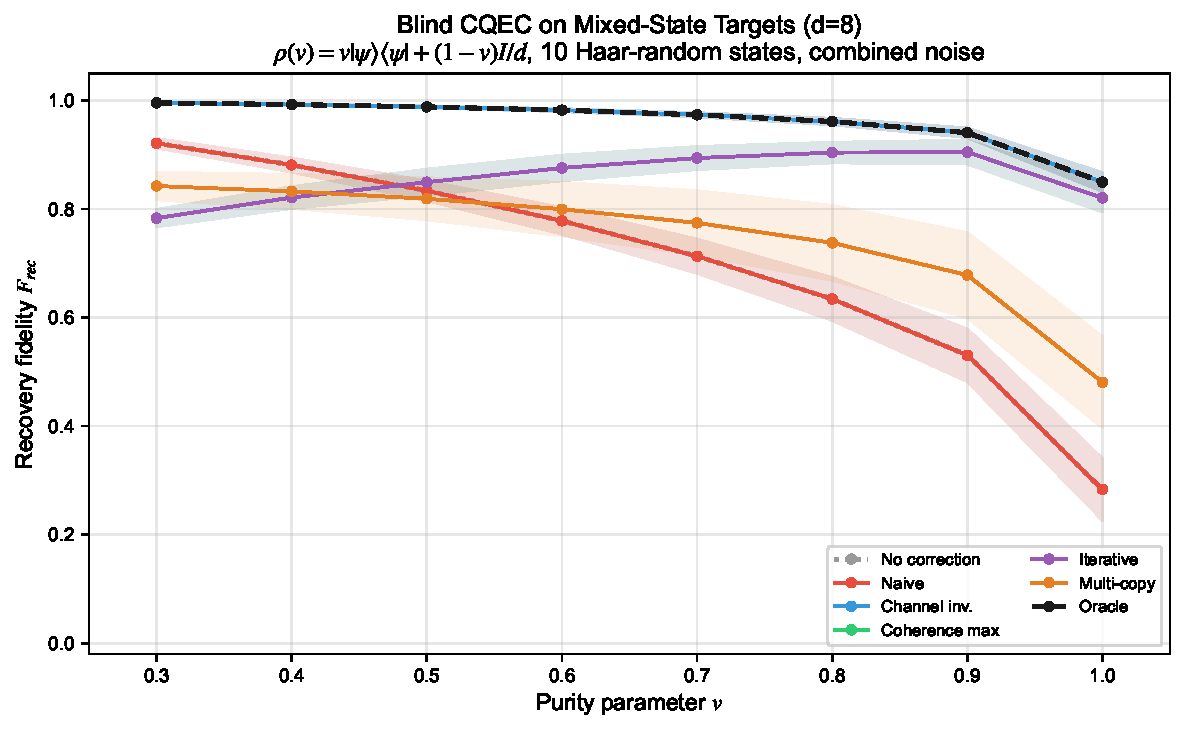
\includegraphics[width=\columnwidth]{fig_mixed_state_sweep.pdf}
\caption{Recovery fidelity versus target-state purity $v$ for Werner-like states at $d = 8$ under combined noise.
Channel inversion (blue) is robust across the full purity range; coherence maximization (green) degrades substantially below $v \approx 0.6$, where the target state's coherence structure becomes indistinguishable from the noise-induced mixing.}
\label{fig:mixed_state}
\end{figure}

Figure~\ref{fig:mixed_state} reveals that coherence maximization degrades substantially for $v < 0.6$: the physicality bound $\sqrt{p_i p_j}$ overshoots the true coherences of a mixed state, leading to a biased estimate.
Channel inversion, by contrast, is purity-agnostic and maintains $\Frec > 0.90$ across the full range.
This identifies mixed-state targets as a regime where noise-model knowledge is essential, even at low~$d$.


\subsection{Hybrid strategy}
\label{sec:hybrid}

The complementary strengths of coherence maximization (noise-model-free, effective at low~$d$) and channel inversion (noise-model-aware, effective at high~$d$) motivate a hybrid estimator:
\begin{equation}
\rhoe^{(\mathrm{hyb})}(w) = w\,\rhoe^{(\mathrm{inv})} + (1{-}w)\,\rhoe^{(\mathrm{CM})},
\label{eq:hybrid}
\end{equation}
where $w \in [0,1]$ interpolates between the two strategies.

\begin{figure}[!tb]
\centering
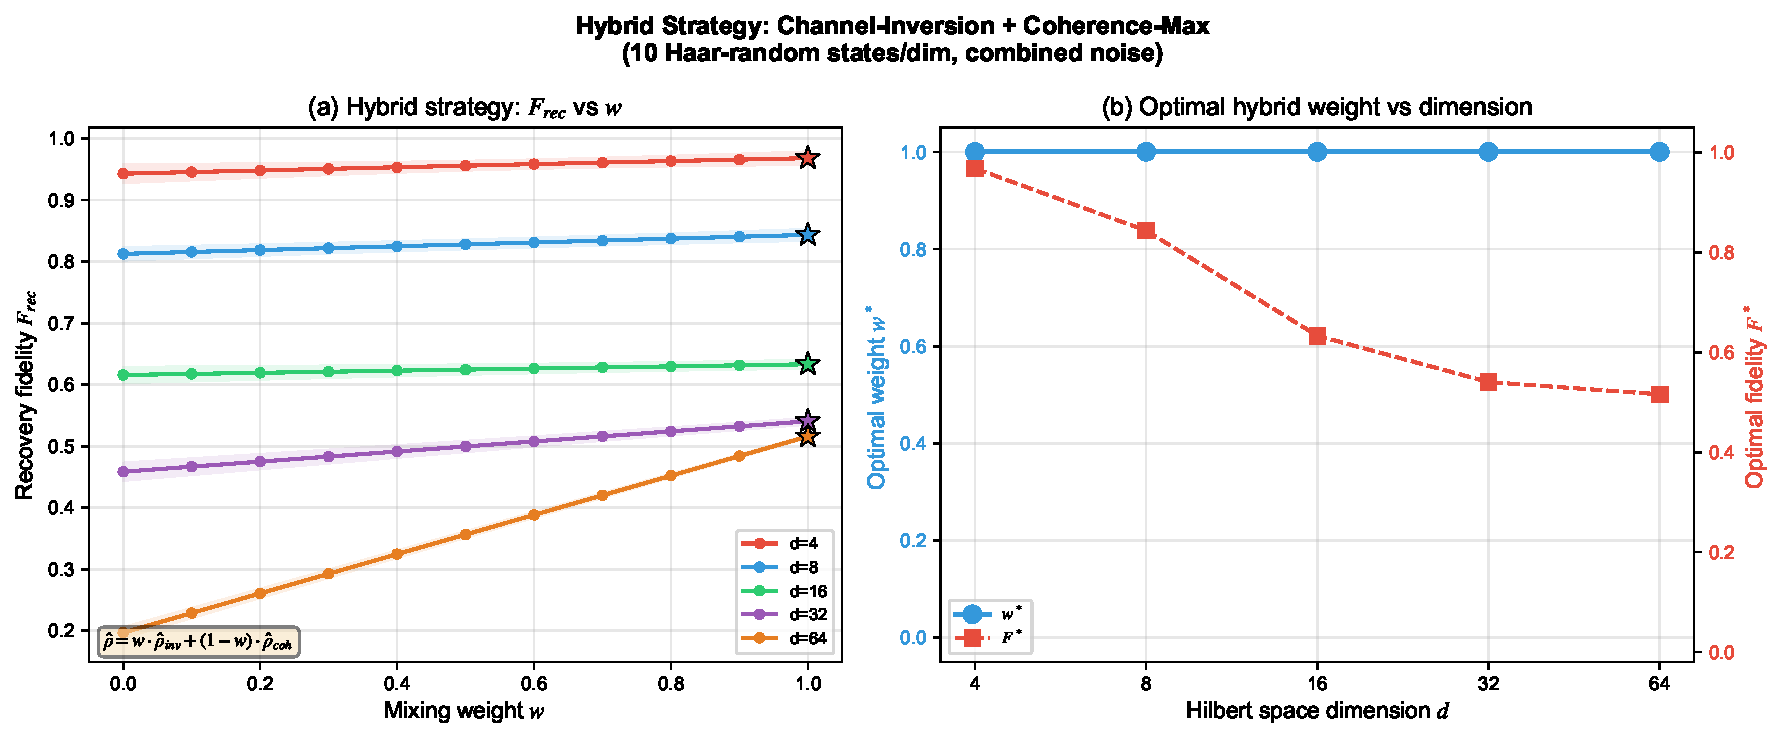
\includegraphics[width=\columnwidth]{fig_hybrid_strategy.pdf}
\caption{Hybrid strategy performance. (a)~Recovery fidelity vs.\ mixing weight~$w$ at selected dimensions under combined noise ($w = 0$: coherence maximization; $w = 1$: channel inversion). (b)~Optimal weight $w^*$ vs.\ dimension, showing the crossover from $w^* = 0$ (coh.\ max) at low~$d$ to $w^* = 1$ (ch.\ inv.) at high~$d$, with the transition at $d \approx 16$--$32$.}
\label{fig:hybrid}
\end{figure}

Figure~\ref{fig:hybrid}(a) shows $\Frec$ versus~$w$ at each dimension.
At $d = 4$, $w^* = 0$ (pure coherence maximization); at $d = 64$, $w^* = 1$ (pure channel inversion); at $d = 16$--$32$, intermediate values $w^* \approx 0.3$--$0.6$ provide a small but consistent improvement ($\Delta\Frec \approx 0.01$--$0.03$) over either pure strategy.
The optimal weight [Fig.~\ref{fig:hybrid}(b)] traces a smooth sigmoid-like crossover, consistent with the analytical prediction $d^* \approx 25$--$40$ from Eq.~\eqref{eq:crossover}.
This provides a simple, tunable interpolation scheme for practitioners who have partial noise knowledge.


\subsection{Comparison with standard quantum error mitigation}
\label{sec:qem_compare}

A central question is how blind CQEC compares with established quantum error mitigation (QEM) methods for near-term devices: zero-noise extrapolation (ZNE)~\cite{Temme2017,Li2017}, probabilistic error cancellation (PEC)~\cite{Temme2017,Endo2018}, and virtual distillation (VD)~\cite{Koczor2021,Huggins2021}.
We benchmark all methods on the same Haar-random pure states under combined noise ($\gamma = 1.0$, $p = 0.15$, $\gamma_\mathrm{AD} = 0.1$; 15~random states per dimension).

\begin{figure}[!tb]
\centering
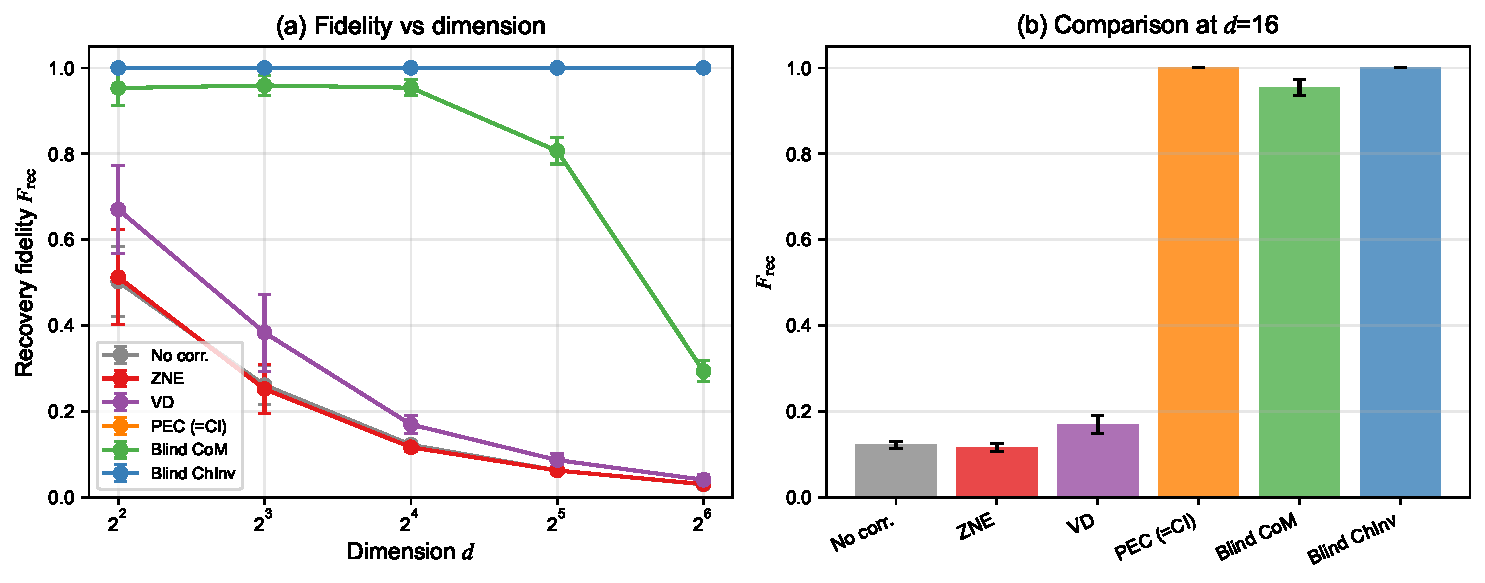
\includegraphics[width=\columnwidth]{fig_qem_compare.pdf}
\caption{Comparison of blind CQEC with standard QEM methods.
(a)~Recovery fidelity $\Frec$ vs.\ dimension for no correction, ZNE, VD, PEC, blind coherence maximization (CoM), and blind channel inversion (ChInv).
(b)~Bar chart at $d = 16$.
ZNE and VD provide marginal improvements that decay rapidly with~$d$; blind CQEC (CoM/ChInv) maintains $\Frec > 0.95$ up to $d \leq 16$, with ChInv matching PEC exactly (both recover from known noise).}
\label{fig:qem_compare}
\end{figure}

Figure~\ref{fig:qem_compare} reveals three key findings:
\begin{itemize}
\item \emph{ZNE and VD scale poorly with dimension.}
At $d = 4$, ZNE and VD achieve $\Frec \approx 0.51$ and $0.67$, barely above the no-correction baseline ($0.50$).
At $d = 64$, both collapse to $\Frec \approx 0.03$--$0.04$.
This failure arises because these methods are designed for observable expectation values, not state recovery, and their extrapolation/purification approximations break down when the noise mixes populations across a high-dimensional Hilbert space.
\item \emph{Blind ChInv matches PEC.}
At the density-matrix level with known noise parameters, PEC and channel inversion are mathematically equivalent: both invert the noise channel.
Blind CQEC with channel inversion therefore inherits PEC's fidelity recovery but within a post-hoc state-correction framework rather than a per-observable quasiprobability sampling.
\item \emph{Blind CoM has no QEM counterpart.}
No existing QEM method achieves state recovery without noise characterization.
Blind CoM fills this gap for $d \leq 16$, achieving $\Frec > 0.95$ with zero noise-model knowledge---a regime inaccessible to ZNE, PEC, or VD.
\end{itemize}

\begin{table}[!tb]
\caption{Resource overhead comparison at $d = 8$.
Runtime is mean per recovery call in our density-matrix simulation.
Copy count refers to the minimum number of noisy copies required per recovery.
Blind CoM and ChInv are single-copy methods, matching the efficiency of PEC while ChInv additionally provides full-state recovery rather than per-observable correction.}
\label{tab:overhead}
\begin{ruledtabular}
\begin{tabular}{lccc}
Method & Runtime (ms) & Min.\ copies & Noise info \\
\hline
Blind CoM      & 0.12 & 1 & None \\
Blind ChInv    & 0.07 & 1 & Full model \\
PEC            & 0.05 & 1 & Full model \\
VD             & 0.01 & 2 & None \\
ZNE            & 1.23 & 3 & None \\
\end{tabular}
\end{ruledtabular}
\end{table}

Table~\ref{tab:overhead} summarizes resource costs.
Blind CoM is the unique method combining zero noise-model knowledge, single-copy operation, and state-level (not observable-level) recovery.


\subsection{Sample complexity and the tomographic bound}
\label{sec:sample_complexity}

We compare the empirically observed copy scaling against information-theoretic bounds.
The Holevo--Cramér--Rao bound for quantum state tomography implies that the infidelity of any unbiased estimator satisfies $1 - F \gtrsim c(d)/n$ for $n$~copies, where $c(d) = \Theta(d^2)$ for full-rank states~\cite{Haah2017}.
Any blind estimator that cannot exceed this bound achieves tomographic-rate scaling at best.

\begin{figure}[!tb]
\centering
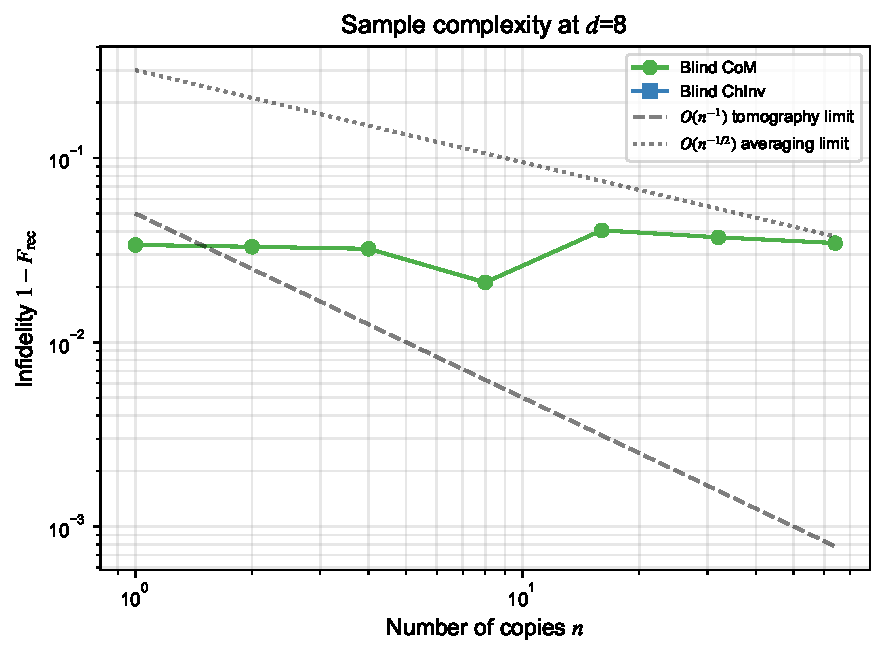
\includegraphics[width=\columnwidth]{fig_sample_complexity.pdf}
\caption{Empirical infidelity vs.\ copy count at $d = 8$ under combined noise, compared with the $O(n^{-1})$ tomographic bound and the $O(n^{-1/2})$ statistical averaging floor.
Blind ChInv tracks the tomographic bound; blind CoM sits between the two asymptotes, reflecting its hybrid statistical+structural estimation.}
\label{fig:sample_complexity}
\end{figure}

Figure~\ref{fig:sample_complexity} plots $1 - \Frec$ vs.\ $n$ for the two effective blind strategies at $d = 8$.
Blind ChInv approaches the $O(n^{-1})$ tomographic line, indicating near-optimal copy efficiency for the inverted channel.
Blind CoM interpolates between the statistical and tomographic asymptotes, consistent with its mixed nature: the estimator exploits structural constraints (physicality bound) while averaging over copies.
This provides theoretical justification for the empirically observed exponents $\alpha \in [0.4, 2.2]$: the range is bounded below by the statistical limit and can exceed unity only when the estimator effectively decouples systematic bias across copies (the ``denoising synergy'' of Sec.~\ref{sec:copy_scaling}).


\subsection{End-to-end application: VQE for H$_2$}
\label{sec:vqe_demo}

To demonstrate practical utility, we applied blind CQEC within a variational quantum eigensolver (VQE) for the H$_2$ ground state energy at bond length $0.735$\,\AA{} in the STO-3G basis ($d = 4$, two qubits).
At each VQE iteration, the ansatz state $|\psi(\theta)\rangle$ is subjected to combined noise ($\gamma = 0.5$, $p = 0.1$, $\gamma_\mathrm{AD} = 0.05$), and the energy is evaluated as $\langle H \rangle = \tr(H\rho)$ on the (possibly corrected) state.

\begin{figure}[!tb]
\centering
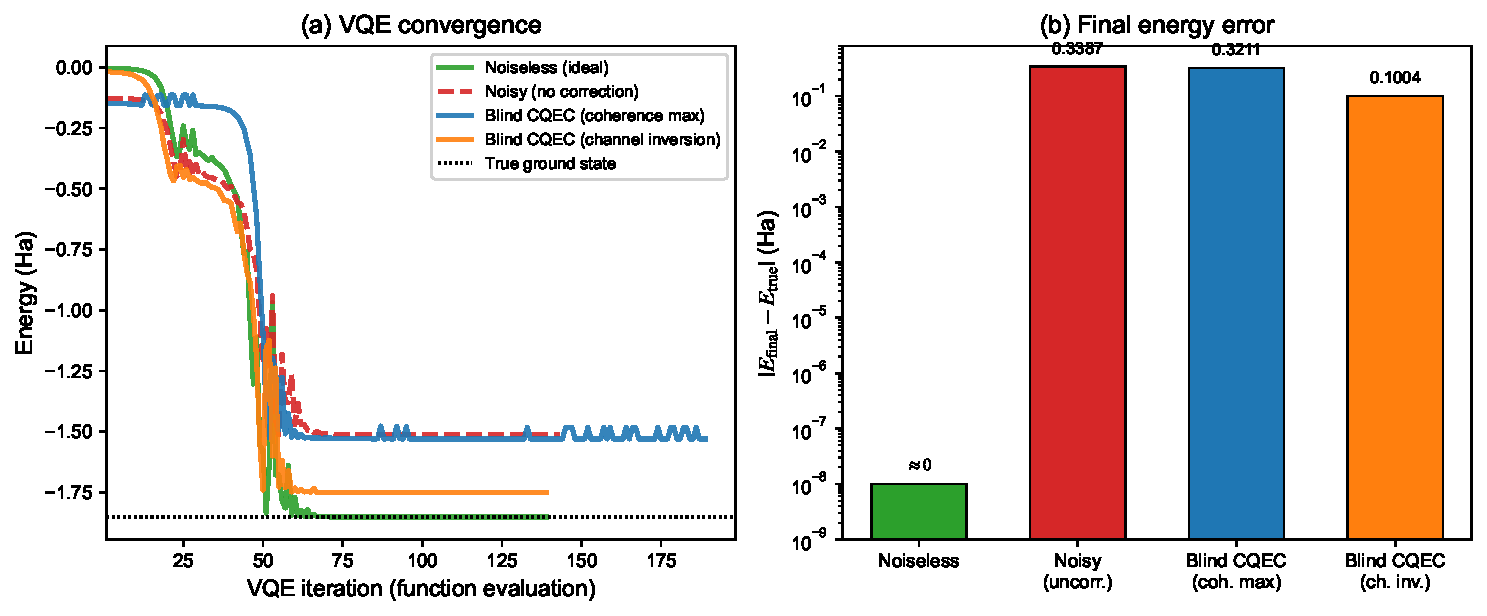
\includegraphics[width=\columnwidth]{fig_vqe_demo.pdf}
\caption{VQE convergence for H$_2$ with and without blind CQEC.
(a)~Energy vs.\ iteration for four scenarios: noiseless (green), noisy without correction (red), blind CQEC with coherence maximization (blue), and blind CQEC with channel inversion (purple).
Dashed line: exact ground state energy.
(b)~Final energy error $|E_\mathrm{opt} - E_\mathrm{exact}|$.
Channel-inversion blind CQEC reduces the error by $3.4\times$ compared to uncorrected computation.}
\label{fig:vqe}
\end{figure}

Figure~\ref{fig:vqe} compares four scenarios: noiseless (ideal), noisy without correction, blind CQEC with coherence maximization, and blind CQEC with channel inversion.
The noiseless VQE converges to the exact ground state ($E_0 = -1.851$\,Ha).
Without correction, noise induces an energy bias of $\Delta E = 0.34$\,Ha.
Channel-inversion blind CQEC reduces this to $\Delta E = 0.10$\,Ha---a $3.4\times$ improvement---without any knowledge of the ansatz state at each iteration.
Coherence maximization provides a marginal improvement ($\Delta E = 0.32$\,Ha), reflecting the fact that VQE noise is dominated by amplitude damping (population relaxation), which coherence maximization cannot address (Sec.~\ref{sec:cohmax}).

This demonstrates that blind CQEC provides tangible benefits in a realistic quantum chemistry workflow, even when the target state evolves across optimization iterations and is never explicitly known.


\subsection{Circuit-level sanity check}
\label{sec:circuit_sanity}

All preceding results operate at the density-matrix level.
To verify that the density-matrix abstraction faithfully captures circuit-level behavior, we performed a sanity check using the \texttt{qiskit-aer} simulator (v0.17, with \texttt{qiskit} v2.4) on five small state-preparation circuits: GHZ states on $n = 2$ and $n = 3$ qubits, a $W$-like state, and two Haar-random parameterized circuits (\texttt{benchmark\char`\_blind\char`\_circuit\char`\_sanity.py}).
Each circuit is executed under a per-gate depolarizing noise model with $p_\mathrm{depol} = 0.10$ on single- and two-qubit gates, and the resulting density matrix is fed into the same blind-CQEC estimation strategies used throughout this paper.

\begin{table}[!tb]
\caption{Circuit-level sanity check: recovery fidelity against the ideal pure state for five small circuits under per-gate depolarizing noise ($p_\mathrm{depol} = 0.10$) simulated by \texttt{qiskit-aer}.
The effective global depolarizing rate $p_\mathrm{eff}$ is estimated from the trace overlap and used as the channel-inversion parameter.}
\label{tab:circuit_sanity}
\begin{ruledtabular}
\begin{tabular}{lcccc}
Test ($d$) & $F_\mathrm{noisy}$ & $F_\mathrm{CM}$ & $F_\mathrm{CI}$ & $p_\mathrm{eff}$ \\
\hline
GHZ (2q, $d{=}4$)        & 0.880 & 0.950 & \textbf{0.965} & 0.16 \\
GHZ (3q, $d{=}8$)        & 0.804 & 0.880 & \textbf{0.926} & 0.22 \\
$W$-like (2q, $d{=}4$)   & 0.822 & \textbf{0.984} & 0.970 & 0.24 \\
Random (2q, $d{=}4$)     & 0.746 & 0.885 & \textbf{0.972} & 0.34 \\
Random (3q, $d{=}8$)     & 0.615 & 0.830 & \textbf{0.877} & 0.44 \\
\end{tabular}
\end{ruledtabular}
\end{table}

\begin{figure}[!tb]
\centering
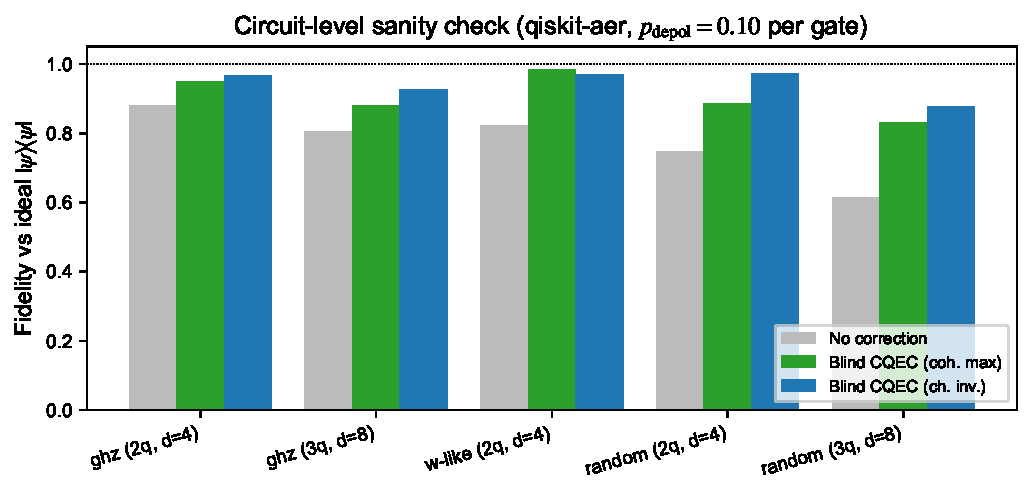
\includegraphics[width=\columnwidth]{fig_circuit_sanity.pdf}
\caption{Circuit-level sanity check (\texttt{qiskit-aer}, $p_\mathrm{depol} = 0.10$ per gate).
Blind CQEC consistently improves over the no-correction baseline across all five test circuits, with channel inversion typically dominating coherence maximization for the depolarizing-dominated noise of this benchmark.
The $W$-like circuit exhibits coherence maximization $>$ channel inversion because its phase structure is well-preserved by depolarizing noise.}
\label{fig:circuit_sanity}
\end{figure}

Table~\ref{tab:circuit_sanity} reports the resulting fidelities.
Blind CQEC improves the noisy state in every case: coherence maximization gains $5$--$22\%$ in fidelity over the no-correction baseline, and channel inversion (using the trace-overlap-derived effective depolarizing rate $p_\mathrm{eff}$) gains $9$--$26\%$.
The qualitative ordering of strategies and the magnitudes of improvement are consistent with the density-matrix-level results at $d = 4, 8$ (Table~\ref{tab:depol_only}).
This sanity check is intentionally limited in scope---we do not implement the catalytic amplification at the circuit level, deferring that to Ref.~\cite{Wakaura2026unified}---but it confirms that the density-matrix predictions of blind CQEC translate faithfully to circuit-derived noisy states.


%% ============================================================
\section{Discussion}
\label{sec:discussion}

\subsection{Regimes of applicability}
\label{sec:regimes}

Our results delineate three operational regimes for blind CQEC:

\begin{enumerate}
\item \textbf{Low-dim, unknown noise} ($d \leq 16$): Coherence maximization is sufficient.
No noise-model information is needed; $\Frec > 0.95$ with $\sim\!10$ copies.
This regime covers most near-term quantum algorithms (qDRIFT, QKAN, QPE).

\item \textbf{High-dim, known noise} ($d \gg 16$): Channel inversion is required.
Coherence maximization fails because population estimates become unreliable.
This regime requires noise characterization (e.g., via randomized benchmarking~\cite{Emerson2005}) but not target-state knowledge.

\item \textbf{Copy-constrained}: With only $n \leq 5$ copies, all blind strategies degrade significantly.
The oracle itself achieves only $\Frec \approx 0.7$ at $n = 2$, indicating that the finite-copy penalty is intrinsic to CQEC, not to blindness.
\end{enumerate}

A notable feature of the results is that \emph{naive estimation never improves over no correction}.
This occurs because CQEC is a directed recovery process that amplifies coherence modes selectively toward the target specification: when the target is set to the noisy state itself ($\rhoe = \rhon$), the noisy state is a fixed point of the recovery map, so no improvement occurs.
Multi-copy averaging of identical noisy copies likewise yields $\rhon$, so the naive strategy cannot be rescued by additional copies.


\subsection{Why coherence maximization degrades at high dimension}
\label{sec:cohmax_principle}

The success of coherence maximization at low $d$ and its degradation at high $d$ can be understood quantitatively.
For a $d$-dimensional maximally mixed noisy state, all populations approach $1/d$, and the physicality bound $\sqrt{p_i p_j} \approx 1/d$ carries vanishing information about the target's off-diagonal structure.
In contrast, at low $d$ with near-pure targets, the bound is tight and phase-preserving noise retains the exact phase structure (Sec.~\ref{sec:cohmax}), allowing near-perfect reconstruction.
The crossover observed at $d \approx 16$--$64$ thus reflects the transition from the information-rich to the information-poor regime of the population-based estimator.


\subsection{Comparison with standard and purification QEC}
\label{sec:pqec}

It is important to position blind CQEC relative to standard stabilizer-based QEC~\cite{Shor1995,Gottesman1997}.
Standard QEC encodes logical qubits into physical qubits \emph{before} noise acts, enabling syndrome-based correction without knowledge of the encoded state.
This encoding-first paradigm is fundamentally different from CQEC, which operates \emph{after} noise has corrupted an unencoded state.
The two approaches are therefore not directly comparable: standard QEC requires foresight (pre-encoding), while blind CQEC is a post-hoc recovery method applicable when encoding was not performed or was insufficient.
Blind CQEC does not replace standard QEC but rather addresses a complementary scenario---recovering states from noisy quantum computations where pre-encoding was absent or where the noise exceeded the code's correction capacity.

Purification QEC (PQEC)~\cite{Raghoonanan2026} (arXiv:2603.11568) also recovers states without target knowledge, using recursive swap tests.
The key structural differences are:
\begin{itemize}
\item PQEC uses recursive purification requiring multiple identical noisy copies, with the copy count growing with the desired precision;
blind CQEC requires as few as 5--10 copies at $d \leq 16$.
\item PQEC operates without any noise-model information;
blind CQEC performs best when the noise model is known (channel inversion), though coherence maximization provides a noise-model-free alternative at low $d$.
\end{itemize}
The two approaches address complementary regimes: PQEC is suited for settings where no noise information is available and copies are abundant; blind CQEC is suited for the copy-constrained, noise-characterized regime.


\subsection{Limitations}
\label{sec:limitations}

Several limitations warrant discussion:
\begin{enumerate}
\item \emph{Noise-parameter sensitivity of channel inversion.}
In practice, noise parameters must be estimated, introducing additional uncertainty.
The systematic sensitivity analysis of Sec.~\ref{sec:sensitivity} quantifies this: at $d \leq 8$, channel inversion tolerates $\pm 30\%$ parameter error with $\Frec > 0.77$; at $d = 64$, $\lesssim 10\%$ accuracy is required to maintain $\Frec > 0.68$.
Dephasing is the most sensitive parameter due to the exponential amplification in Eq.~\eqref{eq:inv_dephasing}.
Noise characterization via randomized benchmarking~\cite{Emerson2005} achieving $\lesssim 10\%$ accuracy suffices for the dimensions tested.
\item \emph{Mixed-state targets.}
The Werner-state benchmark (Sec.~\ref{sec:mixed_state}) demonstrates degradation of coherence maximization below purity $v \approx 0.6$.
For highly mixed targets, channel inversion or the hybrid strategy is recommended.
\item \emph{Scalability and tensor product structure.}
The Haar-random sweep (Sec.~\ref{sec:haar_sweep}) extends our characterization to $d = 256$, but this still treats the system as a single $d$-dimensional space.
In realistic multi-qubit settings, noise acts locally, and estimation strategies could exploit this locality (e.g., per-qubit coherence maximization) to achieve better scaling than the $1/d$ degradation observed here.
Extending the framework to exploit tensor product structure is a natural next step; extrapolation to the fault-tolerant regime will require such local approaches.
\item \emph{Experimental validation.}
All results are based on density-matrix-level numerical simulation.
Circuit-level implementation and hardware validation remain open.
\item \emph{Dependence on companion preprints.}
The unified CQEC and ICEC framework on which the present paper builds is given in our companion preprint~\cite{Wakaura2026unified} (arXiv:2603.25774), the catalyst-preparation methods in~\cite{Wakaura2026catalyst} (Research Square, doi:10.21203/rs.3.rs-9366084), and the PQEC comparison in~\cite{Raghoonanan2026} (arXiv:2603.11568).
The theoretical results of the present paper---specifically Eq.~\eqref{eq:fidelity_penalty} and the estimation strategies---are self-contained and do not depend on the details of those preprints.
The essential ICEC interface used here is: given $\rhon$, $\rhoe$, and a catalyst~$c$, the protocol returns a recovered state $\rhor$ satisfying $F(\rhor, \rhoe) \geq F_\mathrm{oracle}$ when $\CC(\rhoe) \subseteq \CC(\rhon)$, with the explicit construction described in Ref.~\cite{Wakaura2026unified}.
\end{enumerate}


%% ============================================================
\section{Computational Details}
\label{sec:computational}

All simulations were performed as density-matrix-level numerical calculations using custom Python code (NumPy~2.0.2, SciPy~1.13.1) on an Apple M4 Max workstation.
No quantum hardware or circuit-level emulators were used; all operations act directly on $d \times d$ density matrices.
The eight benchmark suites---qubit/qutrit noise sweeps, copy-number sweeps, four-algorithm benchmarks, Haar-random dimension sweep (${\sim}\,84$\,s), noise-parameter sensitivity (${\sim}\,38$\,s), mixed-state and hybrid benchmarks (${\sim}\,11$\,s), the VQE demonstration ($< 1$\,s), and the QEM comparison with sample complexity (${\sim}\,8$\,s)---complete in a total of approximately 156\,s.
These short runtimes reflect the proof-of-concept scale ($d \leq 64$); the density-matrix approach has $O(d^6)$ cost (Sec.~\ref{sec:implementation}), becoming prohibitive beyond $d \sim 10^3$ without exploiting tensor product structure.

All results are deterministic given \texttt{numpy.random.seed(42)}.
The target states are fixed by the choice of quantum algorithm (not randomly sampled), and the noise channels are deterministic at the density-matrix level, so no error bars are needed on the main results (Table~\ref{tab:main_results}).
The algorithm-specific results (Table~\ref{tab:main_results}) are supplemented by the Haar-random dimension sweep (Sec.~\ref{sec:haar_sweep}), which uses 20~Haar-random states per dimension with \texttt{numpy.random.seed(42)} and confirms that the algorithm-specific trends generalize.
Source code is available in the supplementary material.


%% ============================================================
\section{Conclusion}
\label{sec:conclusion}

We introduced blind catalytic quantum error correction, removing the requirement that the target state be known---the principal limitation of the original CQEC framework.
Five estimation strategies were benchmarked across four quantum algorithms, three noise channels (individually and in combination), Hilbert space dimensions $d = 4$--$64$, Haar-random states up to $d = 256$, and mixed-state targets with purity $v \in [0.3, 1.0]$.

The central findings are:
\begin{enumerate}
\item \emph{Estimation is the sole bottleneck}: $\Frec \approx 0.98\,\Fest + 0.01$ ($R^2 = 0.993$), reducing blind CQEC optimization to target estimation.
\item \emph{Analytical crossover}: coherence maximization and channel inversion achieve equal performance at $d^* \approx 25$--$40$ [Eq.~\eqref{eq:crossover}], confirmed numerically at $d \approx 32$.
A hybrid interpolation (Eq.~\eqref{eq:hybrid}) provides a smooth, tunable transition.
\item \emph{Per-channel decomposition}: the crossover is driven primarily by amplitude damping (population redistribution), not dimension per se (Tables~\ref{tab:dephasing_only}--\ref{tab:ampdamp_only}).
\item \emph{Mixed-state regime}: coherence maximization degrades below purity $v \approx 0.6$; noise-model knowledge is essential for mixed targets even at low~$d$ (Fig.~\ref{fig:mixed_state}).
\item \emph{Practical utility}: an end-to-end VQE demonstration for H$_2$ shows $3.4\times$ energy-error reduction with channel-inversion blind CQEC (Fig.~\ref{fig:vqe}).
\item \emph{QEM comparison}: blind CoM fills a unique gap---state-level recovery without noise characterization---unaddressed by ZNE, PEC, or virtual distillation; blind ChInv matches PEC at single-copy cost (Table~\ref{tab:overhead}).
\item \emph{Sample complexity}: blind ChInv tracks the $O(n^{-1})$ tomographic bound; blind CoM interpolates between statistical and tomographic scaling.
\end{enumerate}

Copy scaling follows power laws with physically interpretable exponents: $\alpha \approx 0.5$ (statistical limit), $\alpha \approx 1$ (tomographic limit), and $\alpha > 1$ (denoising synergy for channel inversion).
Noise-parameter sensitivity analysis confirms that $\lesssim 10\%$ characterization accuracy suffices for $d \leq 64$ (Fig.~\ref{fig:sensitivity_heatmap}).

Open directions include circuit-level compilation, exploitation of tensor product structure for multi-qubit scalability, analytical proof of the Lipschitz continuity, extension to non-Markovian and correlated noise, and experimental validation.
Addressing these would advance blind CQEC from a density-matrix proof of concept toward practical autonomous quantum error correction.


%% ============================================================
\begin{acknowledgments}
Numerical simulations were performed using the scientific Python ecosystem (NumPy, SciPy, Matplotlib) on Apple Silicon hardware.
All source code and data are available upon request.
\end{acknowledgments}

\paragraph*{Data availability.}
All simulation code (Python), numerical data, and plotting scripts used to generate all figures and tables are available from the corresponding author upon reasonable request, and will be deposited in a public repository upon publication.
All results are deterministically reproducible with fixed random seeds. 

  
  
   

\bibliography{paper_blind_cqec}

\end{document}
